% ******************************************************** %
%              TEMPLATE DE INFORME ORGA2 v0.1              %
% ******************************************************** %
% ******************************************************** %
%                                                          %
% ALGUNOS PAQUETES REQUERIDOS (EN UBUNTU):                 %
% ========================================
%                                                          %
% texlive-latex-base                                       %
% texlive-latex-recommended                                %
% texlive-fonts-recommended                                %
% texlive-latex-extra?                                     %
% texlive-lang-spanish (en ubuntu 13.10)                   %
% ******************************************************** %
\documentclass[a4paper]{article}
\usepackage[spanish]{babel}
\usepackage[utf8]{inputenc}
\usepackage{charter}   % tipografia
\usepackage{graphicx}
%\usepackage{makeidx}
\usepackage{paralist} %itemize inline
\usepackage{algorithm}  % implementacion ondas en C
% sudo apt-get install texlive-science
\usepackage{algorithmic} % implementacion ondas en C
%\usepackage{float}
\usepackage{amsmath, amsthm, amssymb}
%\usepackage{amsfonts}
%\usepackage{sectsty}
%\usepackage{charter}
%\usepackage{wrapfig}
%\usepackage{listings}
%\lstset{language=C}
% \setcounter{secnumdepth}{2}
\usepackage{underscore}
\usepackage{caratula}
\usepackage{url}

% ********************************************************* %
% ~~~~~~~~              Code snippets             ~~~~~~~~~ %
% ********************************************************* %
\usepackage{color} % para snipets de codigo coloreados
\usepackage{fancybox}  % para el sbox de los snipets de codigo
\definecolor{litegrey}{gray}{0.94}
\newenvironment{codesnippet}{%
	\begin{Sbox}\begin{minipage}{\textwidth}\sffamily\small}%
	{\end{minipage}\end{Sbox}%
		\begin{center}%
		\vspace{-0.4cm}\colorbox{litegrey}{\TheSbox}\end{center}\vspace{0.3cm}}

% ********************************************************* %
% ~~~~~~~~         Formato de las páginas         ~~~~~~~~~ %
% ********************************************************* %
\usepackage{fancyhdr}
\pagestyle{fancy}
%\renewcommand{\chaptermark}[1]{\markboth{#1}{}}
\renewcommand{\sectionmark}[1]{\markright{\thesection\ - #1}}
\fancyhf{}
\fancyhead[LO]{Sección \rightmark} % \thesection\ 
\fancyfoot[LO]{\small{Romera, Tucci, Soliz}}
\fancyfoot[RO]{\thepage}
\renewcommand{\headrulewidth}{0.5pt}
\renewcommand{\footrulewidth}{0.5pt}
\setlength{\hoffset}{-0.8in}
\setlength{\textwidth}{16cm}
%\setlength{\hoffset}{-1.1cm}
%\setlength{\textwidth}{16cm}
\setlength{\headsep}{0.5cm}
\setlength{\textheight}{25cm}
\setlength{\voffset}{-0.7in}
\setlength{\headwidth}{\textwidth}
\setlength{\headheight}{13.1pt}
\renewcommand{\baselinestretch}{1.1}  % line spacing
% ******************************************************** %

\begin{document}

\thispagestyle{empty}
\materia{Organización del Computador II}
\submateria{Segundo Cuatrimestre de 2014}
\titulo{Trabajo Práctico II}
\subtitulo{subtitulo del trabajo}
\integrante{Joaquin Romera }{183/16}{joakromera@gmail.com}
\integrante{Santiago Tucci}{682/16}{stucci4@gmail.com}
\integrante{Carlos Soliz}{406/12}{rcarlos.cs@gmail.com}

\maketitle

\newpage

\thispagestyle{empty}
\vfill
\thispagestyle{empty}
\vspace{3cm}

\tableofcontents
\newpage

\section{Introducción}
En el presente trabajo hicimos un primer acercamiento al modelo de ejecución SIMD (Single instruction Multiple Data). Diseñado como una extensión al set de instrucciones de la arquitectura x86 e introducido por Intel en 1999, esta técnica de paralelización puede mejorar notablemente la performance de un sistema en contextos de programación donde se deben aplicar algoritmos repetitivos sobre un mismo conjunto de datos. Esto lo hace particularmente útil para procesamientos multimedia -audio, video e imágenes- donde la reproducción en tiempo real es crítica. Gracias a las instrucciones SIMD podemos ejecutar una misma operación sobre muchos datos al mismo tiempo en una sola instrucción, contrario a realizarlo en un modelo exclusivamente SISD (single instruction single data). Como veremos a lo largo del trabajo su utilización introducirá notables mejoras en performance y eficiencia de nuestros algoritmos siempre que sea posible su aplicación.

\begin{center}
  \begin{tabular}{cccc}
    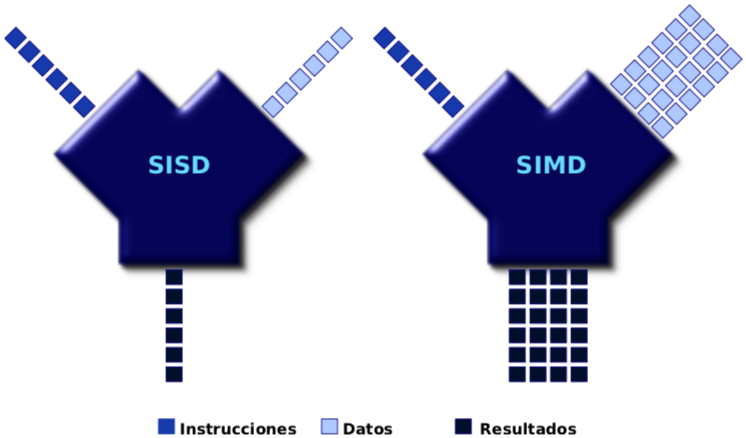
\includegraphics[width=0.45\textwidth]{imagenes/sisdsimd.png} &
    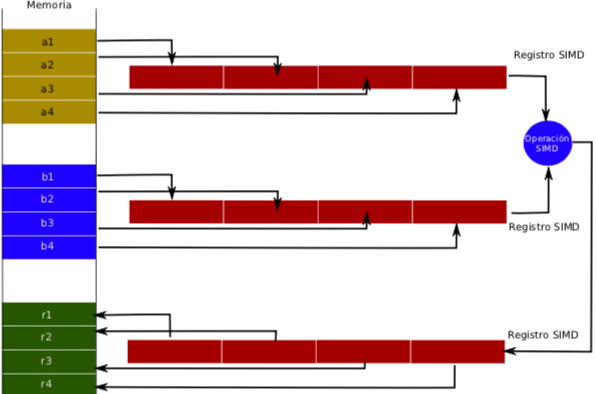
\includegraphics[width=0.45\textwidth]{imagenes/registrossimd.png}\\
  \end{tabular}
 \end{center}

\subsection{Objetivos Generales}
Además de la exploración del modelo SIMD se repasaron conceptos y técnicas de programación vectorizada en C y ASM dentro del campo de aplicación del procesamiento de imagenes. Para esto se llevó a cabo la implementación de los siguientes filtros para imágenes:

\begin{center}
 \begin{tabular}{cccc}
   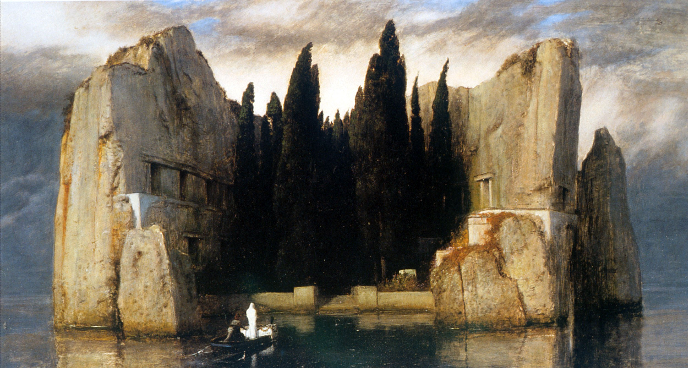
\includegraphics[width=0.2\textwidth]{imagenes/island.png} &
   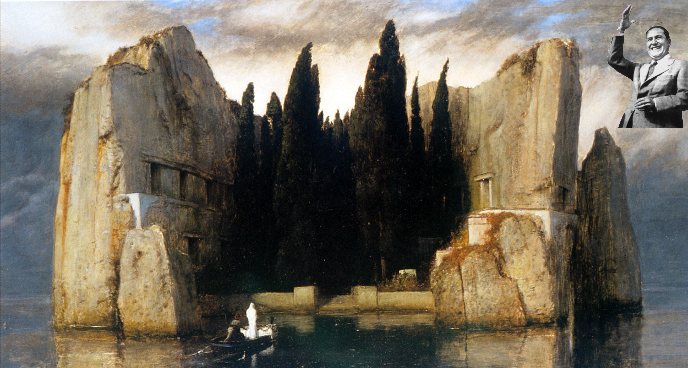
\includegraphics[width=0.2\textwidth]{imagenes/island-blit.png} &
   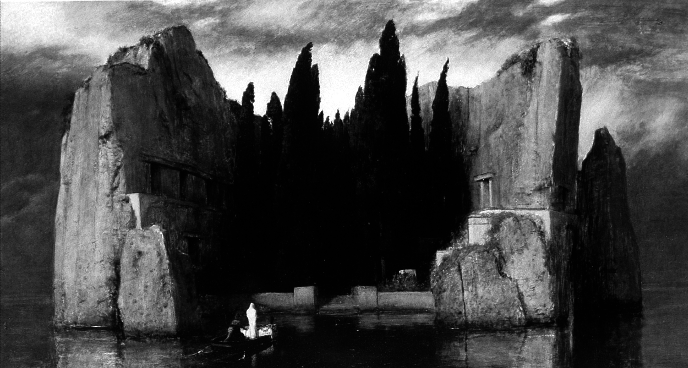
\includegraphics[width=0.2\textwidth]{imagenes/island-monocromatizar.png} \\
   Imagen original & Blit & Monocromatizar \\
   \\
   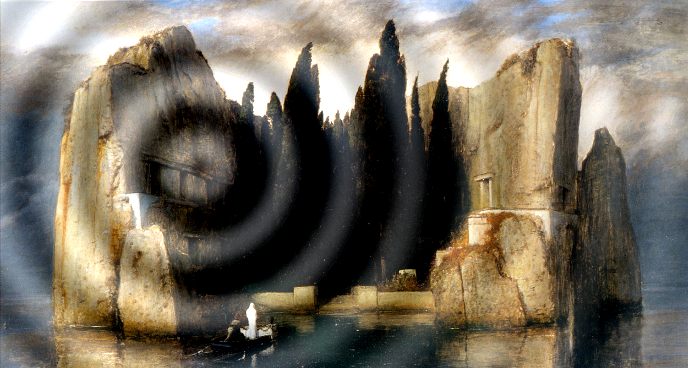
\includegraphics[width=0.2\textwidth]{imagenes/island-ondas.png} &
   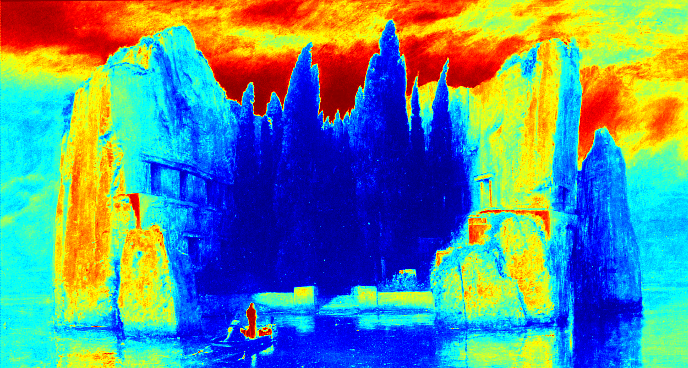
\includegraphics[width=0.2\textwidth]{imagenes/island-temperature.png} &
   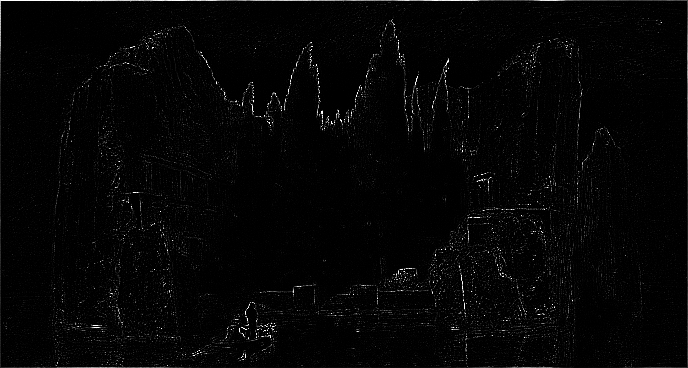
\includegraphics[width=0.2\textwidth]{imagenes/island-edge.png} \\
   Ondas & Temperature & Edge \\
 \end{tabular}
\end{center}

\subsection{Metodología}
La elaboración del trabajo se dividió en dos etapas. En primer lugar, se implementaron ambos filtros tanto en lenguaje C como en lenguaje ensamblador para la arquitectura x86-64 de Intel. En este último caso, se utilizaron las instrucciones SSE de dicha arquitectura, que aprovechan el ya mencionado modelo SIMD para procesar datos en forma paralela.

Una vez realizadas estas implementaciones, fueron sometidas a un proceso de comparación para extraer conclusiones acerca de su rendimiento. Con este fin, se experimentó con variaciones tanto en los datos de entrada como en detalles implementativos de los mismos algoritmos. De esta manera, se pudo recopilar datos sobre el comportamiento de cada implementación, y contrastar estos resultados con diversas hipótesis previamente elaboradas.

A continuación introducimos los filtros y sus respectivas implementaciones, luego describimos los tests realizados y los resultados obtenidos, y finalmente a partir de estos datos otorgamos algunas conclusiones sobre la experiencia realizada.
\newpage

\section{Filtros}
\subsection{Blit}

\subsubsection{Descripción}

Esta operación recibe dos imagenes -original y blit- y genera una nueva combinando ambas. La combinación se realiza considerando un determinado color del blit como transparente para que en el resultado final algunos píxeles del blit queden por encima de la imagen original. En el lugar de aquellos que no son interpretados como transparentes quedan los píxeles del original. La imagen obtenida es una superposición de ambas, teniendo transparencias en el blit siempre que el color del píxel sea igual a (255,0,255).

% \begin{center}
% 	\begin{tabular}{cccc}
% 	  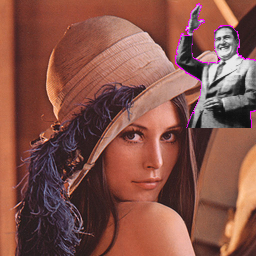
\includegraphics[width=0.2\textwidth]{imagenes/lenaBLIT.jpg} \\
% 	\end{tabular}
%    \end{center}

\begin{multicols}{2}
A pedido de la cátedra la imagen \textbf{blit} ser\'a una foto de Per\'on. La misma será ubicada en la esquina superior derecha de la imagen, además la imagen original deberá tener un tamaño mayor a 89 píxeles de ancho por 128 de alto para poder ubicar el blit. Como resultado tendremos una imagen \textit{Peronizada} cuando se aplique la siguiente función para cada p\'ixel $p$ en la imagen de Per\'on (blit):\\
\begin{center}
	\begin{tabular}{cccc}
	  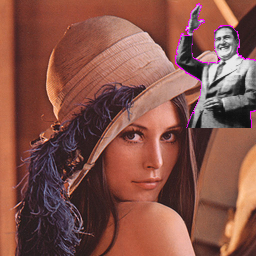
\includegraphics[width=0.3\textwidth]{imagenes/lenaBLIT.jpg} \\
	\end{tabular}
   \end{center}
\end{multicols}

$dst(p) = \begin{cases}
    src(p) & \mathrm{si \;} blit(p) \mathrm{\; es \; de \; color \; magenta, \; es \; decir \; sus \; colores \; son \;} (255, 0, 255)\\
    blit(p) & \mathrm{si \; no}
\end{cases}$ \\

\subsubsection{Implementación C}

Nuestra implementación en C consiste en dos etapas: primero copiamos los píxeles la imagen original en la imagen destino, luego copiamos los píxeles del blit siempre que los mismos no tengan el color (255,0,255). Como Perón debe estar arriba a la derecha de la imagen final, restamos el tamaño de su imagen al de la original en las dimensiones correspondientes. A continuación el pseudocódigo describe el algoritmo:

\begin{algorithm}[H]
  \begin{algorithmic}[1]
		\FORALL{y:=0 \TO  Height($I_{src}$)}		
			\FORALL{x:=0 \TO  Width($I_{src}$)}
			  \STATE $pixel \gets I_{src}(x,y)$ 
			  \STATE $I_{dst}(x,y) \gets pixel$
			\ENDFOR
		\ENDFOR
		\STATE $Int$ $ bh \gets $ Height($I_{src}$) $-$ Height($I_{blit}$)
		\STATE $Int$ $ bw \gets $ Width($I_{src}$) $-$ Width($I_{blit}$)
		 \FORALL{y:=0 \TO  Height($I_{blit}$)}
			\FORALL{x:=0 \TO  Width($I_{blit}$)}
			  	\STATE $pixel \gets I_{blit}(x,y)$
				\STATE $Int$ $ r \gets Red(pixel) $
			  	\STATE $Int$ $g \gets Green(pixel)$
			  	\STATE $Int$ $ b \gets Blue(pixel)$
				\IF{$\neg ( r = 255$ \AND $g = 0$ \AND $b=255)$}
					\STATE $I_{dst}(x+bw,y+bh) = I_{blit}(x+bw,y+bh)$ 
				\ENDIF
			\ENDFOR
		 \ENDFOR
  \end{algorithmic}
  \caption{$blit (I_{src}, I_{dst}, I_{blit})$}
  \label{alg:blit}
\end{algorithm}


\subsubsection{Implementación ASM}

En este filtro procesamos de a 4 píxeles: tenemos dos ciclos, uno que recorre las columnas de la imagen y otra que recorre las filas. Cuando nos encontramos en la fila "Height($I_{src}$) $-$ Height($I_{blit}$)" y la columna "Width($I_{src}$) $-$ Width($I_{blit}$)" es en este momento que tenemos que evaluar si aplicar o no el blit según la fórmula explicada arriba. Abajo detallaremos esta parte del código ASM que desarrolla el blit con un ejemplo.	

\begin{itemize}

	\item En los registros \textbf{xmm0,xmm14} tenemos la copia de los cuatro píxeles que levantamos de memoria, uno es $I_{src}$ y el otro $I_{blit}$ respectivamente.
			Y en \textbf{xmm2, xmm15} las máscaras que utilizamos para la comparación y las operaciones lógicas.

		\begin{center}
		   \begin{tabular}{| c | c | c | c || c | c | c | c || c | c | c | c || c | c | c | c |}
			 \hline
			 a & b & g & r & a & b & g & r & a & b & g & r & a & b & g & r \\ \hline
		   \end{tabular}
		   \\ \textbf{xmm0 $\gets$ $I_{src}$ }
		\end{center}

		\begin{center}
		   \begin{tabular}{| c | c | c | c || c | c | c | c || c | c | c | c || c | c | c | c |}
			 \hline
			 A & B & G & R & A & B & G & R & A & B & G & R & A & B & G & R \\ \hline
		   \end{tabular}
		   \\ \textbf{xmm14 $\gets$ $I_{blit}$ }
		\end{center}
		
		 
		\begin{center}
		   \begin{tabular}{| c | c | c | c || c | c | c | c || c | c | c | c || c | c | c | c |}
			 \hline
			 255 & 255 & 0 & 255 & 255 & 255 & 0 & 255 & 255 & 255 & 0 & 255 & 255 & 255 & 0 & 255 \\ \hline
		   \end{tabular}
		   \\  \textbf{Máscara Magenta xmm15 (maskMagenta)}
		\end{center}

		\begin{center}
		   \begin{tabular}{| c | c | c | c || c | c | c | c || c | c | c | c || c | c | c | c |}
			 \hline
			 00h & 00h & 00h & 00h & 00h & 00h & 00h & 00h & 00h & 00h & 00h & 00h & 00h & 00h & 00h & 00h \\ \hline
		   \end{tabular}
		   \\ \textbf{Máscara en xmm2 (maskCeros)}
		\end{center}
		
	\item Máscara para filtrar píxeles de valor magenta. Suponemos que hay dos píxeles color magenta en $I_{blit}$ a modo de ejemplo en los píxeles 1 y 3 (siguiendo el order de píxel_15,...,píxel_0). A esta máscara la guardamos en xmm12 y xmm15.
	
		\begin{center}
		   \begin{tabular}{| c | c | c | c || c | c | c | c || c | c | c | c || c | c | c | c |}
			 \hline
			 0xFF & 0xFF & 0xFF & 0xFF & 0x00 & 0x00 & 0x00 & 0x00 & 0xFF & 0xFF & 0xFF & 0xFF & 0x00 & 0x00 & 0x00 & 0x00 \\ \hline
		   \end{tabular}
		   \\ \textbf{xmm12,xmm15 $\gets$ pcmpeqd xmm15, xmm14}
		\end{center}

	\item Máscara para filtrar píxeles que no son magenta.

		\begin{center}
		   \begin{tabular}{| c | c | c | c || c | c | c | c || c | c | c | c || c | c | c | c |}
			 \hline
			 0x00 & 0x00 & 0x00 & 0x00 & 0xFF & 0xFF & 0xFF & 0xFF & 0x00 & 0x00 & 0x00 & 0x00 & 0xFF & 0xFF & 0xFF & 0xFF \\ \hline
		   \end{tabular}
		   \\ \textbf{xmm15 $\gets$ pcmpeqd xmm15, xmm13}
		\end{center}

	\item  Me quedo con los valores de $I_{src}$ que tengo que poner en la imagen $I_{dst}$.
		\begin{center}
		   \begin{tabular}{| c | c | c | c || c | c | c | c || c | c | c | c || c | c | c | c |}
			 \hline
			 A & B & G & R & 0x00 & 0x00 & 0x00 & 0x00 & A & B & G & R & 0x00 & 0x00 & 0x00 & 0x00 \\ \hline
		   \end{tabular}
		   \\ \textbf{xmm12 $\gets$ pand xmm12, xmm0}
		\end{center}		

	\item Me quedo con los valores de $I_{blit}$ que tengo que poner en la imagen $I_{dst}$.
		\begin{center}
		   \begin{tabular}{| c | c | c | c || c | c | c | c || c | c | c | c || c | c | c | c |}
			 \hline
			 0x00 & 0x00 & 0x00 & 0x00 & a & b & g & r & 0x00 & 0x00 & 0x00 & 0x00 & a & b & g & r \\ \hline
		   \end{tabular}
		   \\ \textbf{xmm15 $\gets$ pand xmm15, xmm14}
		\end{center}		
	
	\item Junto todos los valores en XMM15.
		\begin{center}
		   \begin{tabular}{| c | c | c | c || c | c | c | c || c | c | c | c || c | c | c | c |}
			 \hline
			 A & B & G & R & a & b & g & r & A & B & G & R & a & b & g & r \\ \hline
		   \end{tabular}
		   \\ \textbf{xmm15 $\gets$ por xmm15, xmm12}
		\end{center}		
	\item Por último resta guardar estos 4 píxeles (XMM15) en $I_{dst}$.

\end{itemize}

Para más detalles dejamos un extracto del código ASM:

\begin{codesnippet}
\begin{verbatim}
	maskMagenta: db 255	 ,0, 255, 255, 255, 0, 255, 255, 255, 0, 255, 255, 255, 0, 255, 255
	maskCero: db 0, 0, 0, 0, 0, 0, 0, 0, 0, 0, 0, 0, 0, 0, 0, 0 

section .text

blit_asm:
		...
		movdqu xmm0, [rdi]; xmm0=|A B G R|A B G R|A B G R|A B G R|; img	
		movdqu xmm14, [r15]; xmm14=|a b g r|a b g r|a b g r|a b g r|; blit

							   ;Filtramos los valores color magenta
		pcmpeqd xmm15, xmm14   ; xmm15=|FF FF FF FF|00 00 00 00|FF FF FF FF|00 00 00 00| 
		movdqu xmm12, xmm15	   ; xmm12= xmm15 paso la mascara a xmm12 

							   ;Filtramos los valores que no son magenta
		pcmpeqd xmm15, xmm13   ; xmm15=|00 00 00 00|FF FF FF FF|00 00 00 00|FF FF FF FF|

							   ;Conservamos con los velores de xmm0 para poner en la imagen
		pand xmm12, xmm0       ; xmm2=|A B G R|00 00 00 00|A B G R|00 00 00 00|

							   ;Nos quedamos con los valores de blit para en la imagen
		pand xmm15, xmm14      ; xmm15=|00 00 00 00|a b g r|00 00 00 00|a b g r|
		
							   ; Juntamos los dos valores en xmm15
		por xmm15, xmm12 	   ;xmm15=|A B G R|a b g r|A B G R|a b g r|
		movdqu [rsi], xmm15	   ; Escribimos en el destino
		movdqu xmm15, [maskMagenta]
		movdqu xmm13, [maskCero]
		...
\end{verbatim}
\end{codesnippet}
\subsection{Monocromatizar}

\subsubsection{Descripción}

\begin{wrapfigure}{r}{0.3\textwidth}
	\centering
	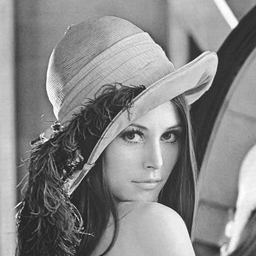
\includegraphics[width=0.3\textwidth]{imagenes/lenaMONO.jpg}
\end{wrapfigure}

El objetivo de este filtro es convertir una imagen color a una escala de grises. A diferencia de otros filtros, los pixeles de la imagen de salida estarán compuestos por un solo byte, que representará la intensidad de la luz. El criterio para obtener este valor es tomar el máximo entre los componentes R, G, B originales de cada pixel y aplicarlo al correspondiente en la imagen destino. Para esto aplicamos, a todos los pixeles de la imagen original, la siguiente función:

\begin{center}
	$I_{out}(p) = max(R, G, B)$
\end{center}

\hfill

\subsubsection{Implementación C}

A continuación el pseudocódigo de la implementación en C:

\begin{algorithm}[H]
  \begin{algorithmic}[1]
		\FORALL{y:=0 \TO  Height($I_{src}$)}
		 %\FOR x:=0 \TO  Width($I_{src}$)\STEP 1 \DO
			\FORALL{x:=0 \TO  Width($I_{src}$)}
			  \STATE $pixel \gets I_{src}(x,y)$
			  \STATE $Int$ $ r \gets Red(pixel) $
			  \STATE $Int$ $g \gets Green(pixel)$
			  \STATE $Int$ $ b \gets Blue(pixel)$
			  \STATE $Int$ $max \gets max(r, max(g, b))$
			  \STATE $pixel \gets DevolverPixel(r,g,b)$
			  \STATE $I_{dst}(x,y) \gets pixel$
			\ENDFOR
		 \ENDFOR
  \end{algorithmic}
  \caption{$monocromatizar (I_{src}, I_{dst})$}
  \label{alg:monocromatizar}
\end{algorithm}

\subsubsection{Implementación ASM}

En este filtro procesamos de a 4 píxeles en cada iteración usando las instrucciones \textbf{SSE} de la arquitectura. Por cada iteración se realizaron los cálculos del máximo de cada píxel y este se guardó en la imagen de salida.

\begin{itemize}

	\item En los registros \textbf{xmm0,xmm4, xmm5} tenemos la copia de los cuatro píxeles que levantamos de memoria. Y en \textbf{xmm1, xmm2, xmm3} las máscaras que usamos para los shuffles que luego utilizaremos para permutar los componentes.

		\begin{center}
		   \begin{tabular}{| c | c | c | c || c | c | c | c || c | c | c | c || c | c | c | c |}
			 \hline
			 a & b & g & r & a & b & g & r & a & b & g & r & a & b & g & r \\ \hline

		   \end{tabular}
		   \\ \textbf{xmm0, xmm4, xmm5}
		\end{center}
		 
		\begin{center}
		   \begin{tabular}{| c | c | c | c || c | c | c | c || c | c | c | c || c | c | c | c |}
			 \hline
			 15 & 13 & 13 & 13 & 11 & 9 & 9 & 9 & 7 & 5 & 5 & 5 & 3 & 1 & 1 & 1 \\ \hline
		   \end{tabular}
		   \\  \textbf{Mascara en xmm1 (mask1)}
		\end{center}

		\begin{center}
		   \begin{tabular}{| c | c | c | c || c | c | c | c || c | c | c | c || c | c | c | c |}
			 \hline
			 15 & 14 & 14 & 14 & 11 & 10 & 10 & 10 & 7 & 6 & 6 & 6 & 3 & 2 & 2 & 2 \\ \hline
		   \end{tabular}
		   \\ \textbf{Mascara en xmm2 (mask2)}
		\end{center}

		\begin{center}
		   \begin{tabular}{| c | c | c | c || c | c | c | c || c | c | c | c || c | c | c | c |}
			 \hline
			 15 & 12 & 12 & 12 & 11 & 8 & 8 & 8 & 7 & 4 & 4 & 4 & 3 & 0 & 0 & 0 \\ \hline
		   \end{tabular}
		   \\ \textbf{Mascara en xmm3(mask3)}
		\end{center}

	\item Realizamos el \textbf{shuffle xmm4, xmm1} que nos coloca el componente \textbf{g} en las posiciones que podemos observar en el registro xmm4. Y luego calculamos el máximo con la instrucción \textbf{pmaxub}. 

		\begin{center}
		   \begin{tabular}{| c | c | c | c || c | c | c | c || c | c | c | c || c | c | c | c |}
			 \hline
			 a & g & g & g & a & g & g & g & a & g & g & g & a & g & g & g \\ \hline
		   \end{tabular}
		   \\ \textbf{xmm4 $\gets$ pshufb xmm4, xmm1}
		\end{center}


		\begin{center}
		   \begin{tabular}{| c | c | c | c || c | c | c | c || c | c | c | c || c | c | c | c |}
			 \hline
			 a & . & . & max(g,r) & a & . & . & max(g,r) & a & . & . & max(g,r) & a & . & . & max(g,r)  \\ \hline
		   \end{tabular}
		   \\ \textbf{xmm4 $ \gets $ pmaxub xmm4, xmm0}
		\end{center}

	\item Realizamos el mismo procedimiento en este paso. Luego nos quedaría el valor del máximo (ver imagen). 
		\begin{center}
		   \begin{tabular}{| c | c | c | c || c | c | c | c || c | c | c | c || c | c | c | c |}
			 \hline
			 a & b & b & b & a & b & b & b & a & b & b & b & a & b & b & b \\ \hline
		   \end{tabular}
		   \\ \textbf{xmm5 $\gets$ pshufb xmm5, xmm2}
		\end{center}

		\begin{center}
		   \begin{tabular}{| c | c | c | c || c | c | c | c || c | c | c | c || c | c | c | c |}
			 \hline
			 a & . & . & max(g,r,b) & a & . & . & max(g,r,b) & a & . & . & max(g,r,b) & a & . & . & max(g,r,b)  \\ \hline
		   \end{tabular}
		   \\ \textbf{xmm4 $\gets$ pmaxub xmm4, xmm5}
		\end{center}


	\item Solo resta copiar los máximos. Para esto utilizaremos el shuffle junto con la máscara contenida en xmm3.

		\begin{center}
		   \begin{tabular}{| c | c | c | c || c | c | c | c || c | c | c | c || c | c | c | c |}
			 \hline
			 a & max & max & max & a & max & max & max & a & max & max & max & a & max & max & max  \\ \hline
		   \end{tabular}
		   \\ \textbf{xmm5 $\gets$ pshufb xmm4, xmm3}
		\end{center}

\end{itemize}

Por último resta copiar esto a memoria, brindamos el código ASM de este paso.

\begin{codesnippet}
\begin{verbatim}
section .data
	mask1: db 1, 1, 1, 3, 5, 5, 5, 7, 9, 9, 9, 11, 13, 13, 13, 15
	mask2: db 2, 2, 2, 3, 6, 6, 6, 7, 10, 10, 10, 11, 14, 14, 14, 15
	mask3: db 0, 0, 0, 3, 4, 4, 4, 7, 8, 8, 8, 11, 12, 12, 12, 15

section .text

monocromatizar_inf_asm:
	...
	movdqu xmm0, [rdi]; xmm0=|a b g r|a b g r|a b g r|a b g r|
	movdqu xmm4, xmm0; xmm4= xmm0
	movdqu xmm5, xmm0; xmm5= xmm0

	pshufb xmm4, xmm1; xmm4=|a g g g|a g g g|a g g g|a g g g|
	pmaxub xmm4, xmm0; xmm4=|a . . max(g,r)|a . . max(g,r)|a . . max(g,r)|a . . max(g,r)|;1er máximo

	pshufb xmm5, xmm2; xmm5=|a b b b|a b b b|a b b b|a b b b|			
	pmaxub xmm4, xmm5; xmm4=|a . . max(g,r,b)|a . . max(g,r,b)|a . . max(g,r,b)|;máx de máximos
						; xmm4=|a . . max|a . . max|a . . max|a . . max|	
	pshufb xmm4, xmm3; xmm4=|a max max max|a max max max|a max max max|a max max max|

	movdqu [rsi], xmm4; [rsi]= xmm4
	...
\end{verbatim}
\end{codesnippet}
\subsection{Ondas}

\begin{multicols}{2}
  Este filtro combina la imagen original con una imagen de ondas, dando tonos más oscuros y mas claros en forma de onda. Estas se centran en un punto de la imagen -pasado como parámetro- y se expanden hacia sus bordes de manera concéntrica. Para ello aplicamos implementamos el pseudocódigo del algoritmo otorgado por la cátedra, en el cual a cada pixel de la imagen se le suma un valor de profundidad basado en su distancia al centro de las ondas.
  \begin{center}
    \begin{tabular}{cccc}
      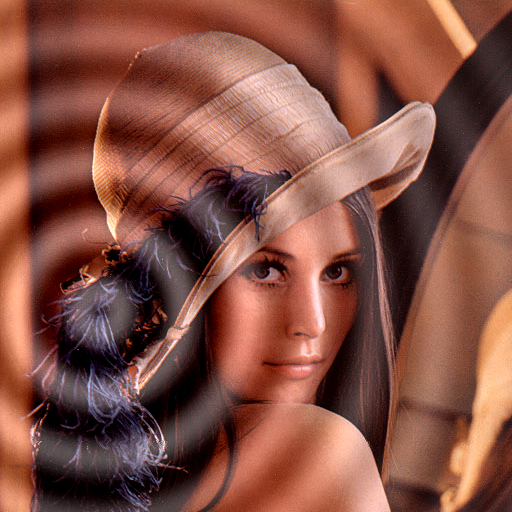
\includegraphics[width=0.3\textwidth]{imagenes/lenaONDA.jpg} \\
    \end{tabular}
     \end{center}
  \end{multicols}

\subsubsection{Implementación C}

Nuestra implementación en C es una traducción iterativa del mencionado algoritmo propuesto por la cátedra en el siguiente pseudocódigo:

\begin{algorithm}[H]
  \begin{algorithmic}[1]
    \FORALL{pixel ubicado en la posici'on $\mathbf{(x, y)}$}
      \STATE $d_x \gets x - x_0$
      \STATE
      \STATE $d_y \gets y - y_0$
      \STATE
      \STATE $d_{xy} \gets \sqrt{d_{x}^2+d_{y}^2}$
      \STATE
      \STATE $r \gets \frac{(d_{xy} - RADIUS)}{WAVELENGTH}$
      \STATE
      \STATE $a \gets \frac{1}{1 + (\frac{r}{TRAINWIDTH})^2 }$
      \STATE
      \STATE $t \gets ( r-floor(r) ) \cdot 2 \cdot \pi - \pi$
      \STATE
      \STATE $prof \gets a \cdot (t - \frac{t^3}{6}+\frac{t^5}{120}-\frac{t^7}{5040})$
      \STATE
      \STATE $pixel = prof \cdot 64 + I_{src}(x, y)$    
      \STATE
      \STATE $I_{dst}(x, y) = saturar(pixel)$
    \ENDFOR
  \end{algorithmic}
  \caption{$ondas (I_{src}, I_{dst}, x_0, y_0)$}
  \label{alg:ondas}
\end{algorithm}

\begin{itemize}
  \item $x_0$ e $y_0$ representan la posici'on donde est'a centrada la onda,
  \item $RADIUS$, $WAVELENGTH$ y $TRAINWIDTH$ son constantes que definen la 
  forma de la onda y
  \item $saturar(x)$ es una funci'on que retorna $0$ si $x$ es menor $0$, $255$
  si es mayor a $255$ y $x$ en cualquier otro caso.
\end{itemize}

\subsubsection{Implementación ASM}
Es este ejercicio procesaremos de a 4 píxeles, por cada iteracion sobre la imagen.
\subsubsection*{Cálculo de la profudidad}
Vamos a dar una breve explicación del cáculo de la profundidad en assembler.

\subsubsection*{caculo de la distancia}

Est este ejecicio queremos calcular la distancia, esto es $\sqrt{(x-x_0)^2+(y-y_0)^2} = \sqrt{dx^2+dy^2}$.
Este proceso lo hacemos con los 4 píxeles juntos.
La idea es obtener en \emph{xmm3=$|(dx3^2+dy3^2)^{1/2}|$...$|(dx0^2+dy0^2)^{1/2}|$}. Podemos observar abajo el detalle de cada calculo e instrucción usada.
\begin{codesnippet}
\begin{verbatim}
                            ;CALCULO DE PROFUNDIDAD
                            ;xmm11=|x_0|x_0|x_0|x_0| Centro de la onda eje x
                            :xmm14=|y_0|y_0|y_0|y_0| Centro de la onda eje y
    movdqu xmm3, xmm11      ;xmm3=|x3|x2|x1|x0| 
    psubd xmm3, xmm13       ;xmm3=|x3-x_0|x2-x_0|x1-x0|x0-x_0|                    x - x_0
							
    movdqu xmm4, xmm12      ;xmm4=|y1|y2|y3|y4|
    psubd xmm4, xmm14       ;xmm4=|y3-y_0|y2-y_0|y1-y_0|y0-y_0|                     y - y_0	
                            ;sabiendo dx3=x3-x_0,dx2=x2-x_0,dx1=x1-x_0 y dx0=x0-x_0
    pmulld xmm3, xmm3       ;xmm3=|dx3^2|dx2^2|dx1^2|dx0^2|
    pmulld xmm4, xmm4       ;xmm4=|dy3^2|dy2^2|dy1^2|dy0^2|
                            ;Realizamos la suma dx^2+dy^2
    paddd xmm3, xmm4        ;xmm3=|dx3^2+dy3^2|...|dx0^2+dy0^2|
                            ; Convertimos de doble word integer a Float
    cvtdq2ps xmm3, xmm3     ;xmm3= Convertimos de doble word integer a Float
                            ;Sacamos raiz cuadrada a cada paquet dobleWord, o sea (dx^2+dy^2)^(1/2)
    sqrtps xmm3, xmm3       ;xmm3=|(dx3^2+dy3^2)^(1/2)|...|(dx0^2+dy0^2)^(1/2)|
\end{verbatim}
\end{codesnippet}


\subsubsection*{Cálculos auxiliares(variables R, K, A y T)}

En esta sección queremos cálcular:

\begin{center}
	$R \gets (dxy-RADIUS)/WAVELENGTH$\\
	$K \gets R-floor(r)$ \\
	$A \gets \frac{1.0}{(1.0+(\frac{r}{TRAINWIDTH)}*\frac{r}{TRAINWIDTH))}}$ \\
	$T \gets K*2*PI-PI$
\end{center}

\begin{codesnippet}
\begin{verbatim}
                                ;Calculo de R, o sea (dx*dx+dy*dy)^(1/2) - RADIO 
                                ;xmm9=|RADIO|RADIO|RADIO|RADIO|
    subps xmm3, xmm9            ;xmm3=|dxy3-RADIO|dxy2-RADIO|dxy1-RADIO|dxy0-RADIO| donde dxy es la distancia
                                ;xmm8=|WAVELENGTH|WAVELENGTH|WAVELENGTH|WAVELENGTH|
                                ; R <- ((dx*dx+dy*dy)^(1/2) - RADIO)/WAVELENGTH
    divps xmm3, xmm8            ;xmm3=|R3|R2|R1|R0|	
;###################################################################################
                                ;Calculo de K
    movdqu xmm7, xmm3           ;xmm7=|R3|R2|R1|R0|
    movdqu xmm4, xmm3           ;xmm4=|R3|R2|R1|R0|
                                ;El valor 0001b me permite activar la opcion de TRUNCAR c/u Float
                                ;Donde floor(R) es el el truncamiento
    roundps xmm3, xmm3, 0001b   ;xmm3=|floor(R3)|floor(R2)|floor(R1)|floor(R0)|

                                ;K  <- R - floor(R)
    subps xmm4, xmm3            ;xmm4=|R3-floor(R3)|R2-floor(R2)|R1-floor(R1)|R0-floor(R0)|								
                                ;xmm4=|k3|k2|k1|k0|
                                ;xmm3 <- R
                                ;xmm4 <- K
;######################################################################################
                                ;Cálculo de T
    movdqu xmm5, xmm4           ;xmm5=|k3|k2|k1|k0|
                                ;xmm10=|1|1|1|1| 
    paddd xmm10, xmm10          ;xmm10=|2|2|2|2|
    cvtdq2ps xmm10, xmm10       ;xmm10=|2|2|2|2| convierto a Floats
    mulps xmm5, xmm10           ;xmm5=|k3*2|k2*2|k1*2|k0*2| multiplico por 2 a los k's
    divps xmm10, xmm10          ;xmm10=|1.0|1.0|1.0|1.0| floats
    cvtps2dq xmm10, xmm10       ;xmm10=|1|1|1|1| convertimos de floats a integer
                                ;xmm6=|PI|PI|PI|PI|
    mulps xmm5, xmm6            ;xmm5=|k3*2*PI|k2*2*PI|k1*2*PI|k0*2*PI|
                                ;Queremos realizar lo siguiente  t = k*2*PI-PI
    subps xmm5, xmm6            ;xmm5=|k3*2*PI-PI|k2*2*PI-PI|k1*2*PI-PI|k0*2*PI-PI|
                                ;xmm5=|T3|T2|T1|T0| donde T=k*2*PI-PI 
;######################################################################################
                                ;Calculo de A
    movdqu xmm3, xmm7           ;xmm3=|R3|R2|R1|R0|
                                ;R/TRAINDIWTH
    divps xmm3, xmm15           ;xmm3=|R3/TRAINDIWTH|R2/TRAINDIWTH|R1/TRAINDIWTH|R0/TRAINDIWTH|
                                ;R/TRAINDIWTH * R/TRAINDIWTH
    mulps xmm3, xmm3            ;xmm3=|(R3/TRAINDIWTH)^2|...|(R0/TRAINDIWTH)^2|
    cvtdq2ps xmm10, xmm10       ;xmm10=|1.0|1.0|1.0|1.0| convertimos de Integer a Floats
                                ;1 + (R/TRAINDIWTH * R/TRAINDIWTH)
    addps xmm3, xmm10           ;xmm3=|1 + (R1/TRAINDIWTH)^2|...|1 + (R0/TRAINDIWTH)^2|
    movdqu xmm4, xmm10          ;xmm4= |1.0|1.0|1.0|1.0|
                                ;A = 1 / 1 + (R/TRAINDIWTH * R/TRAINDIWTH)
    divps xmm4, xmm3            ;xmm4=|A3|A2|A1|A0|
\end{verbatim}
\end{codesnippet}

\subsubsection*{Cálculos Sin_Taylor}
En esta parte queremos hacer el cálculos de
\begin{center}
	$SinTaylor \gets (t - \frac{t^3}{6}+\frac{t^5}{120}-\frac{t^7}{5040})$ \\
	$prof \gets A * SinTaylor*64$
\end{center}
Veremos q en $xmm4=|A3*(t3-t3^3/6+t3^5/120-t3^7/5040)*64|...|A1*(t0-t0^3/6+t0^5/120-t0^7/5040)*64|$ el Sin Taylor Buscado.
\begin{codesnippet}
\begin{verbatim}
                            ;sin taylor
    movdqu xmm1, xmm5       ;xmm1=|t3|t2|t1|t0|
                            ;calculamos x al cubo
    movdqu xmm3, xmm5       ;xmm3=|t3|t2|t1|t0|
    mulps xmm3, xmm5        ;xmm3=|t3^2|t2^2|t1^2|t0^2|
    mulps xmm3, xmm5        ;xmm3=|t3^3|t2^3|t1^3|t0^3|	

    movq xmm2, r15          ;xmm2=|0|0|0|6|
    packssdw xmm2, xmm2     ;xmm2=|0|6|0|6|
    packssdw xmm2, xmm2     ;xmm2=|6|6|6|6|
    cvtdq2ps xmm2, xmm2	    ;xmm2=|6|6|6|6| convierto de integer a Floats

    divps xmm3, xmm2        ;xmm3=|(t3^3)/6|(t2^3)/|(t1^3)/6|(t0^3)/6|
    subps xmm1, xmm3        ;xmm1=|t3-(t3^3)/6|t2-(t2^3)/|t1-(t1^3)/6|t0-(t0^3)/6|
                     ...............                  
                            ;Calculamos T a la quinta
                            ;Los calculos son analogos y obtenemos los siguiente
                     ...............
    divps xmm3, xmm2        ;xmm3=|t3^5/120|t2^5/120|t1^5/120|t0^5/120|								
    addps xmm1, xmm3        ;xmm1=|t3-(t3^3)/6+t3^5/120|...|t0-(t0^3)/6+t0^5/120|								
                     ................... 
                            ;Cálculamos T a la septima
                            ;Cálculos analogos
                    ................	
    divps xmm3, xmm2        ;xmm3=|t3^7/5040|t2^7/5040|t1^7/5040|t0^7/5040|
                    
    subps xmm1, xmm3        ;xmm1=|t3-(t3^3)/6+t3^5/120-t3^7/5040|...|t0-(t0^3)/6+t0^5/120-t0^7/5040|

    subps xmm1, xmm3        ;xmm1=|t3-(t3^3)/6+t3^5/120-t3^7/5040|...|t0-(t0^3)/6+t0^5/120-t0^7/5040|								
                    ................
                            ;Cálculamos la multiplicacion por A y por 64
    mulps xmm4, xmm1        ;xmm4=|A3*(t3-t3^3/6+t3^5/120-t3^7/5040)|...|A1*(t0-t0^3/6+t0^5/120-t0^7/5040(|
                            ;Renombramos a xmm4=|prof3|prof2|prof1|prof0|		
    mulps xmm4, xmm8        ;xmm4=|prof3*64|prof2*64|prof1*64|prof0*64|

\end{verbatim}
\end{codesnippet}

\subsubsection*{Agregar profundidad a los pixeles(ultímo paso)}
En este paso ya tenemos el cálculo de la profundidad en el registro $xmm4$, sólamente nos resta agregar la profundidad a los 4 pixeles q estamos por procesar. O sea falta lo siguinte:
\begin{center}
       $pixel \gets prof + I_{src}(x, y)$    
      
      $I_{dst}(x, y) \gets saturar(pixel)$
\end{center}
Abajo muestramos los segmentos mas importantes del codigo que lo resuelve.
\begin{codesnippet}
\begin{verbatim}
    cvtps2dq xmm4, xmm4             ;xmm4=|prof3*64|prof2*64|prof1*64|prof0*64| conviertimos de float a Integer

    movdqu xmm7, xmm4               ;xmm7=|prof3*64|prof2*64|prof1*64|prof0*64|
                                    ;me quedo con el 3er dobleWord usando el shuffle
    pshufd xmm4, xmm4, 11111111b    ;xmm4=|prof3*64|prof3*64|prof3*64|prof3*64|

    pxor xmm3, xmm3
                                    ;Levanto imagen en Xmm1
    movdqu xmm1, [rdi]              ;xmm1=|a3 b3 g3 r3|a2 b2 g2 r2|a1 b1 g1 r1|a0 b0 g0 r0|			
    movdqu xmm0, xmm1               ;xmm0=|a3 b3 g3 r3|a2 b2 g2 r2|a1 b1 g1 r1|a0 b0 g0 r0|
    punpckhbw xmm1, xmm3            ;xmm1=|a3 b3 g3 r3|a2 b2 g2 r2| de byte a word parte alta
    movdqu xmm2, xmm1               ;xmm2=|a3 b3 g3 r3|a2 b2 g2 r2| 
    punpckhwd xmm1, xmm3            ;xmm1=|a3 b3 g3 r3| de word a DobleWord parte alta
    punpcklwd xmm2, xmm3            ;xmm2=|a2 b2 g2 r2| de word a DobleWord parte baja
    paddd xmm1, xmm4                ;xmm1=|prof3*64+a3|prof3*64+b3|prof3*64+g3|prof3*64+r3|
                                    ;Renombro O(a3)=prof3*64+a3, etc
                                    ;xmm1=|O(a3) O(b3) O(g3) O(r3)|
#######################################################
    
    
                                    ; De Manera similar obtenmos xmm2
                                ......................			
    paddd xmm2, xmm4                ;xmm2=|a2+prof2*64|b2+prof2*64|g2+prof2*64|r2+prof2*64|
                                    ;xmm2=|O(a2)|O(b2)|O(g2)|O(r2)|	
                                    ;Empaquetamos de DobleWord a Word	
    packssdw xmm2,xmm1              ;xmm2=|O(a3) O(b3) O(g3) O(r3)|O(a2) O(b2) O(g2) O(r2)|
    movdqu xmm5, xmm2               ;xmm5=|O(a3) O(b3) O(g3) O(r3)|O(a2) O(b2) O(g2) O(r2)|
						.....................
    paddd xmm1, xmm4                ;xmm1=|a1+prof1*64|b1+prof1*64|g1+prof1*64|r1+prof1*64|
                                    ;xmm1=|O(a1)|O(b1)|O(g1)|O(r1)|						
                        .....................
    paddd xmm2, xmm4                ;xmm2=|a0+prof0*64|b0+prof0*64|g0+prof0*64|r0+prof0*64| shuffle posicion 0 de dobleWord
                                    ;xmm2=|O(a0)|O(b0)|O(g0)|O(r0)|                   
                                    ;Empaquetamos de DobleWord a Word
    packssdw xmm2,xmm1              ;xmm2=|O(a1) O(b1) O(g1) O(r1)|O(a0) O(b0) O(g0) O(r0)|						
                                    ;Empaquetamos de Word Byte
    packuswb xmm2,xmm5              ;xmm2=|O(a3) O(b3) O(g3) O(r3)|O(a2) O(b2) O(g2) O(r2)
                                    ;     |O(a1) O(b1) O(g1) O(r1)|O(a0) O(b0) O(g0) O(r0)|                      

    movdqu [rsi], xmm2              ;Cargamos a memoria xmm2                        			
\end{verbatim}
\end{codesnippet}


\subsection{Temperature}

\begin{codesnippet}
\begin{verbatim}
bool between(unsigned int val, unsigned int a, unsigned int b)
{
	return a <= val && val <= b;
}


void temperature_c    (
	unsigned char *src,
	unsigned char *dst,
	int width,
	int height,
	int src_row_size,
	int dst_row_size)
{
    unsigned char (*src_matrix)[src_row_size] = (unsigned char (*)[src_row_size]) src;
    unsigned char (*dst_matrix)[dst_row_size] = (unsigned char (*)[dst_row_size]) dst;

    for (int i_d = 0, i_s = 0; i_d < height; i_d++, i_s++) {
        for (int j_d = 0, j_s = 0; j_d < width; j_d++, j_s++) {
            bgra_t *p_d = (bgra_t*)&dst_matrix[i_d][j_d*4];
            bgra_t *p_s = (bgra_t*)&src_matrix[i_s][j_s*4];
            *p_d = *p_s;
        }
    }

    for(int i = 0; i < height; i++){
        for(int j = 0; j < width * 4; j += 4){
            unsigned char temperature = (unsigned char)((src_matrix[i][j] + src_matrix[i][j + 1] + src_matrix[i][j + 2]) / 3);
            if(temperature < 32){
                dst_matrix[i][j]     = 0;
                dst_matrix[i][j + 1] = 0;
                dst_matrix[i][j + 2] = (unsigned char )(128 + temperature * 4);
            }
            else if(between(temperature,32,95)){
                dst_matrix[i][j] 	 = 0;
                dst_matrix[i][j + 1] = (unsigned char)((temperature - 32) * 4);
                dst_matrix[i][j + 2] = 255;
            }
            else if(between(temperature,96,159)){
                dst_matrix[i][j] 	 = (unsigned char)((temperature - 96) * 4);
                dst_matrix[i][j + 1] = 255;
                dst_matrix[i][j + 2] = (unsigned char)(255 - (temperature - 96) * 4);
            }
            else if(between(temperature,160, 223)){
                dst_matrix[i][j] 	 = 255;
                dst_matrix[i][j + 1] = (unsigned char)(255 - (temperature - 160) * 4);
                dst_matrix[i][j + 2] = 0;
            }
            else{
                dst_matrix[i][j] 	 = (unsigned char)(255 - (temperature - 224) * 4);
                dst_matrix[i][j + 1] = 0;
                dst_matrix[i][j + 2] = 0;
            }
        }
    }
}
\end{verbatim}
\end{codesnippet}

\subsection{Edge}

\subsubsection{Descripción}

\begin{multicols}{2}
El filtro EDGE devuelve una imagen con los bordes de otra imagen original. Esto se logra observando los píxeles donde la intensidad de la imagen cambia de forma abrupta, lo cual puede ser logrado buscando saltos en una función de intensidades. Esta idea de detectar los bordes fue implementada a través del operador de Laplace, cuya matriz es: 

$$ M = \left(
\begin{matrix}
    0.5 & 1 & 0.5 \\
    1 & -6 & 1 \\
    0.5 & 1 & 0.5
\end{matrix}
\right)$$

\begin{center}
	\begin{tabular}{cccc}
		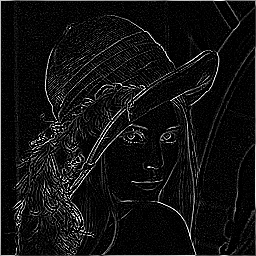
\includegraphics[width=0.3\textwidth]{imagenes/lenaEDGA.jpg} \\
		\end{tabular}
	\end{center}
\end{multicols}

La forma de utilizarla es posicionando uno a uno cada pixel en el centro de la matriz y realizando el siguiente cálculo: 

$$dst(x, y) = \sum_{k = 0}^2 \sum_{l = 0}^2 src(x + k - 1, y + l - 1) * M(k, l)$$

Al igual que monocromatizar, EDGE opera sobre imágenes en escala de grises (1 componente de color por píxel).
Como no se pueden procesar los bordes con la función anterior se aplica la siguiente función: $dst(x, y) = src(x,y)$.

\subsubsection{Implementación C}

Ignorando la primera y la última fila al igual que el primer y el último pixel de cada fila, recorrimos iterativamente todos los pixeles de la imagen realizando el siguiente proceso: por cada pixel calculamos todas las sumas parciales de la función que resulta de la aplicación de la matriz de Laplace, luego todas estas sumas fueron almacenadas en una variable auxiliar (\textit{edge}). Si el valor de \textit{edge} requería ser saturado se lo restringió a los valores 0/255 y finalmente se guardó el resultado en el pixel correspondiente de la imagen destino.

\begin{algorithm}[H]
  \begin{algorithmic}[1]
		\FORALL{y:=1 \TO  Height($I_{src}$$-1$)}
			\FORALL{x:=1 \TO  Width($I_{src}$)$-1$}
			  \STATE $m_{0,0} \gets I_{src}(x-1,y-1)*0.5$
			  \STATE $m_{0,1} \gets I_{src}(x-1,y)*1$
			  \STATE $m_{0,2} \gets I_{src}(x-1,y+1)*0.5$
			  \STATE $m_{1,0} \gets I_{src}(x,y-1)*1$
			  \STATE $m_{1,1} \gets I_{src}(x,y)*(-6)$
			  \STATE $m_{1,2} \gets I_{src}(x,y+1)*1$
			  \STATE $m_{2,0} \gets I_{src}(x+1,y-1)*0.5$
			  \STATE $m_{2,1} \gets I_{src}(x+1,y)*1$
			  \STATE $m_{2,2} \gets I_{src}(x+1,y+1)*0.5$
			  \STATE $edge \gets m_{0,0}+m_{0,1}+m_{0,2}+m_{1,0}+m_{1,1}+m_{1,2}+m_{2,0}+m_{2,1}+m_{2,2}$
			  \STATE $I_{dst}(x,y) \gets Saturar(edge)$
			\ENDFOR
		 \ENDFOR
  \end{algorithmic}
  \caption{$edge (I_{src}, I_{dst})$}
  \label{alg:edge}
\end{algorithm}

\subsubsection{Implementación ASM}
\newpage
\section{Mediciones y Experimentos}

Para poder realizar las mediciones utilizamos la instrucción de assembler \textit{rdtsc}. Con ella podemos obtener el valor de Time Stamp Counter (TSC) del procesador -un registro de 64 bits presente en todos los procesadores x86 desde los Pentium-, como este se incrementa en uno con cada ciclo del procesador podemos obtener la duración en cantidad de ticks de una llamada a una función calculando la diferencia de este registro al principio y al final de su ejecución. Ya que esta medida no es constante entre llamadas, por cada caso de test se realizaron 1000 llamadas y se las promedió utilizando el framework provisto por la cátedra. Para lidiar con los posibles outliers se calculó una media 10\% podada. Otros detalles de las mediciones se dan específicamente por cada experimento producido.

\subsection{Performance}

Nos propusimos observar el crecimiento en la cantidad de ciclos por llamada de cada función a medida que crecía el tamaño del archivo de entrada. Para esto utilizamos la imagen de Lena con tamaños de 16x16 píxeles hasta 1024x1024 en incrementos de a 8 píxeles por lado -para el filtro Blit las mediciones arrancaron con imágenes de 128x128 dadas las restricciones del filtro-. El objetivo de estos tests es comparar la performance de la implementación de cada filtro en un lenguaje de alto nivel como C y en uno de nivel más bajo como Assembler. Sabemos que la programación en bajo nivel provee poca -o ninguna- abstracción del set de instrucciones de una arquitectura, debido a esta cercanía del código con el procesador podríamos esperar que la ejecución sea más rápida y que fuese más eficiente en el uso de la memoria. Por el lado del código en C, hicimos las mediciones compilando con los flags O0 y O3 para observar en mayor detalle las variaciones en performance.

En todos los resultados obtenidos observamos que nuestra implementación en ASM requirió menos ciclos de reloj que su contraparte en C en cualquiera de sus variantes. Al mismo tiempo no observamos diferencias notorias entre compilar el código en C usando los flags O0 y O3, al menos no en comparación a la difererencia con el código en assembly. 

Las diferencias registradas en cada implementación son coherentes con el diseño de los algoritmos dadas las posibilidades de cada paradigma de programación: mientras que en los casos de la programación en alto nivel con C toda la programación la realizamos secuencialmente procesando de a un píxel, en bajo nivel con ASM podemos procesar múltiples píxeles con pocas instrucciones SIMD, acortando significativamente la cantidad de ciclos.

\begin{wrapfigure}{r}{0.3\textwidth}
	\centering
	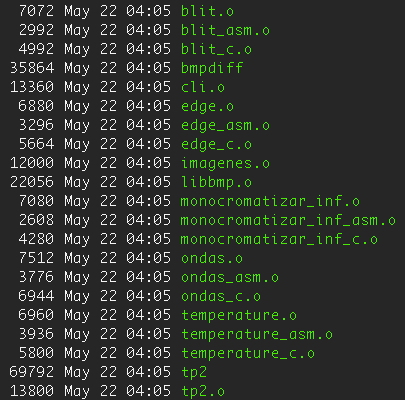
\includegraphics[width=0.3\textwidth]{imagenes/testperformance/sizes.png}
\end{wrapfigure}

También podemos apreciar la diferencia en bytes de los archivos objeto producidos por los compiladores (primera columan de la imagen a la derecha). En todos los casos los archivos generados por GCC son más pesados que los ensamblados por NASM, pesando estos últimos entre un 55\% y un 65\% lo que pesan sus pares en C.

Como ventaja innegable que tiene C por sobre Assembly, o la de cualquier lenguaje de alto nivel por sobre uno de bajo nivel, es la facilidad de uso y debuggeo, su legibilidad, portabilidad, etc. Un ejemplo de esta diferencia es la cantidad de líneas de código que requiere cada algoritmo según el tipo de lenguaje utilizado, llegando nuestras implementaciones en ASM a requerir entre 2 y 5 veces la cantidad de líneas que ocupan en C.

En la página siguiente están los gráficos correspondientes a los filtros y sus mediciones de performance.

\begin{center}
	\begin{tabular}{cccc}
	  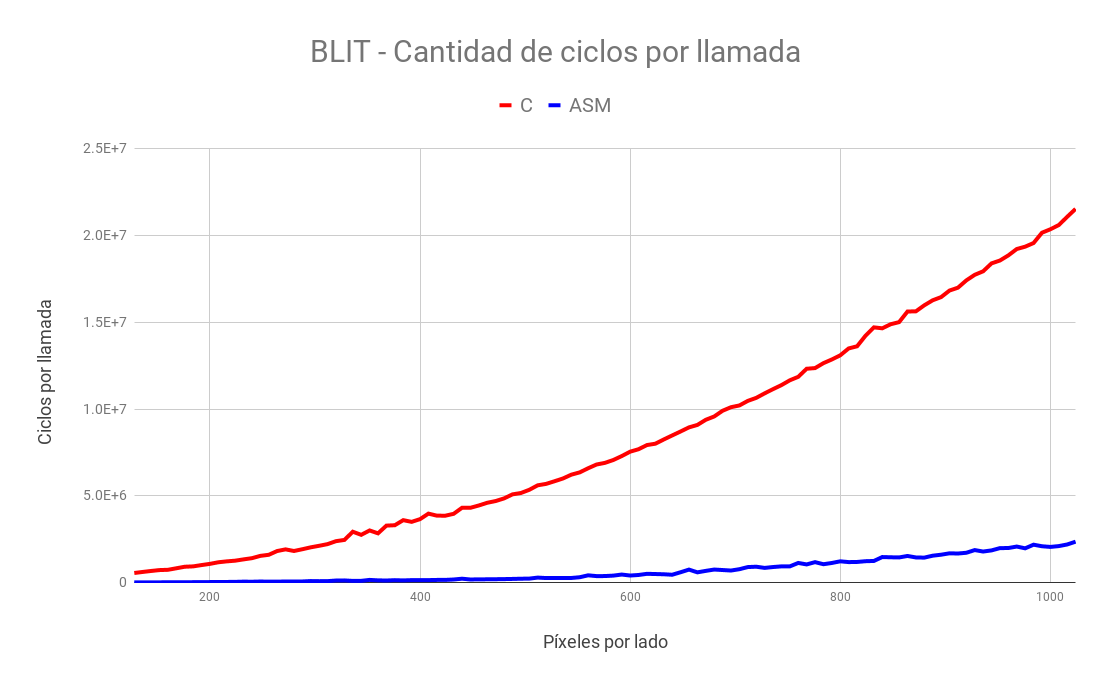
\includegraphics[width=0.45\textwidth]{imagenes/testperformance/BLITperformance.png} &
	  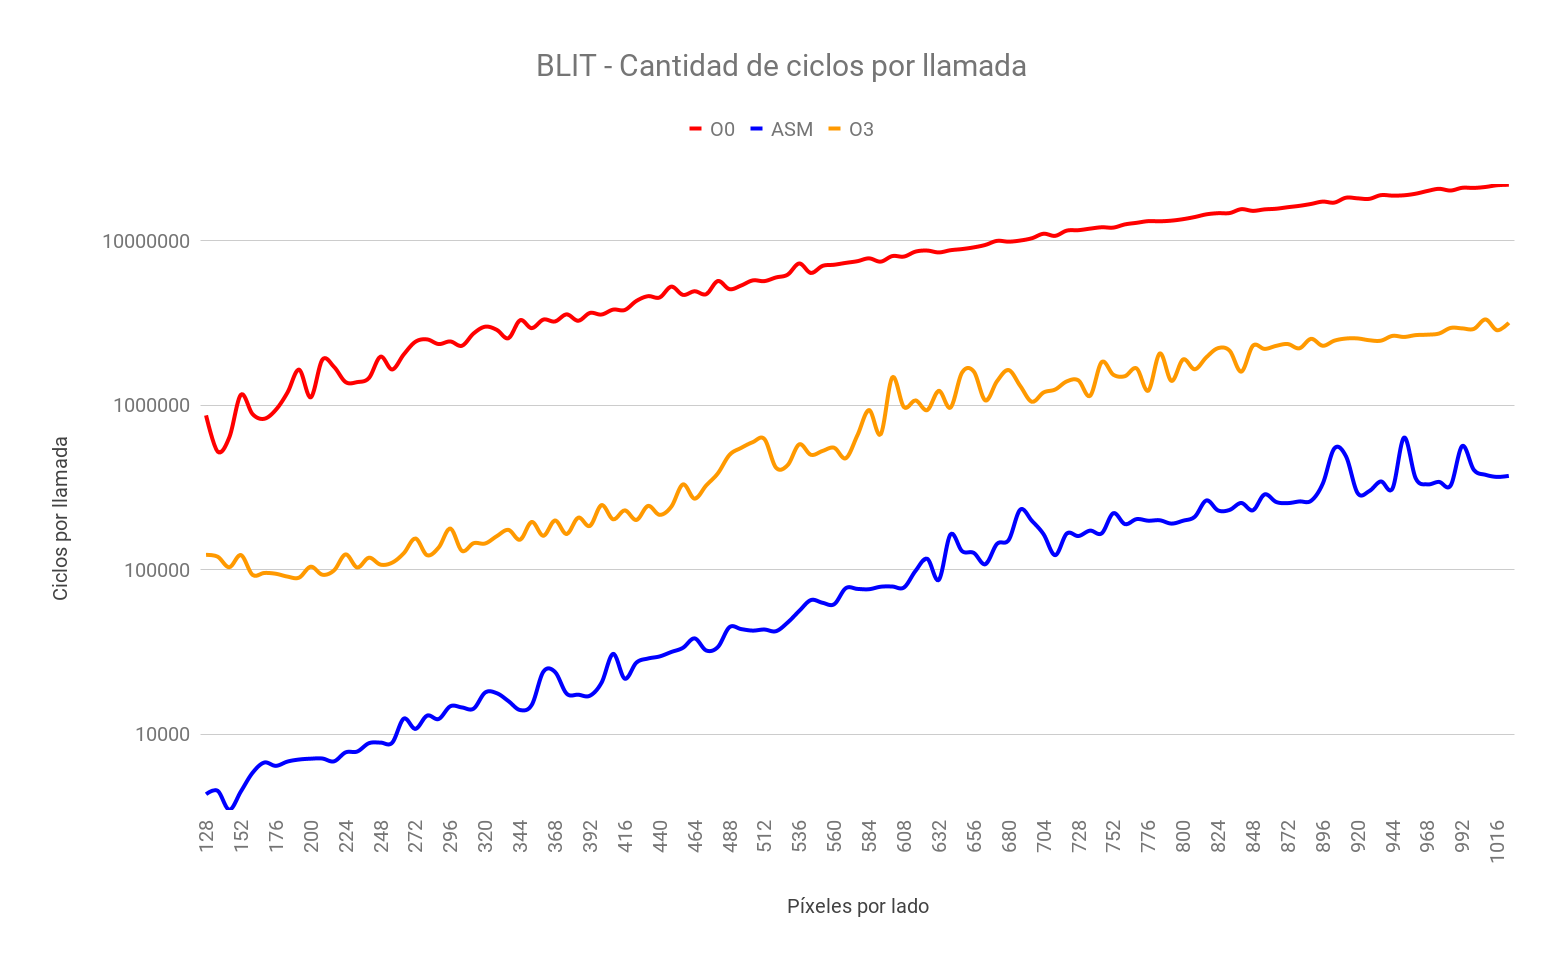
\includegraphics[width=0.45\textwidth]{imagenes/testperformance/BLITperformanceLOG.png} \\
	  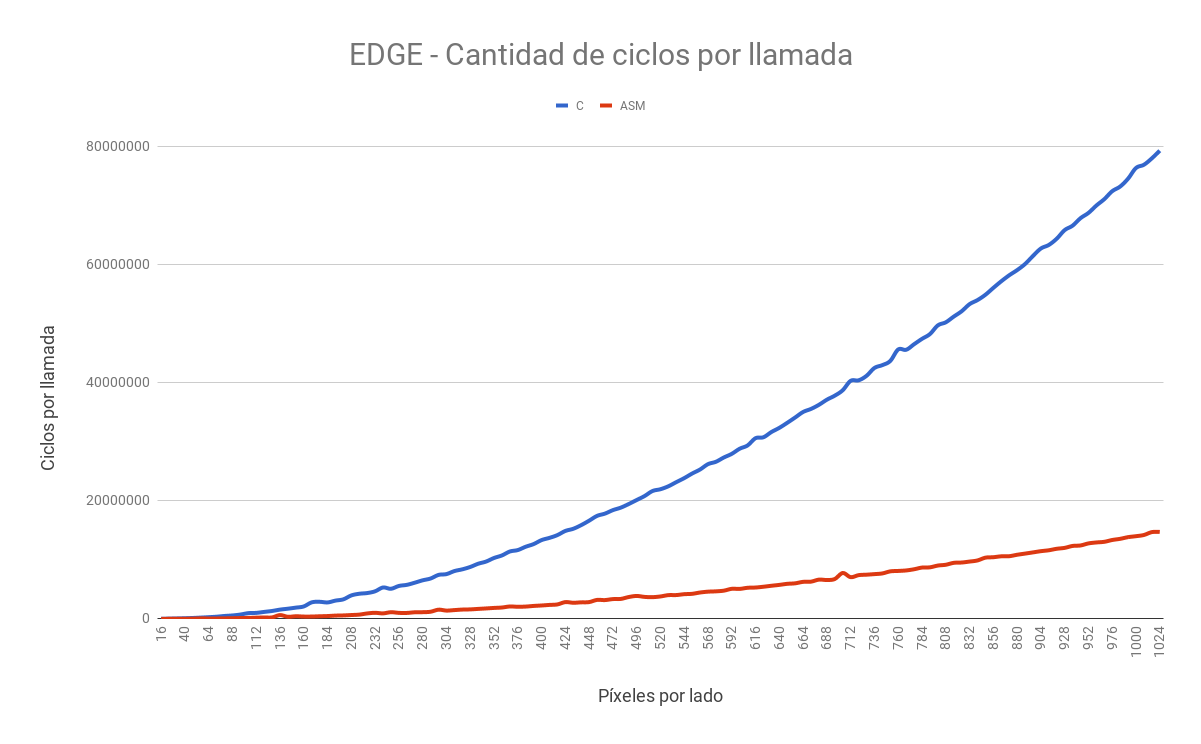
\includegraphics[width=0.45\textwidth]{imagenes/testperformance/EDGEperformanceLIN.png} &
	  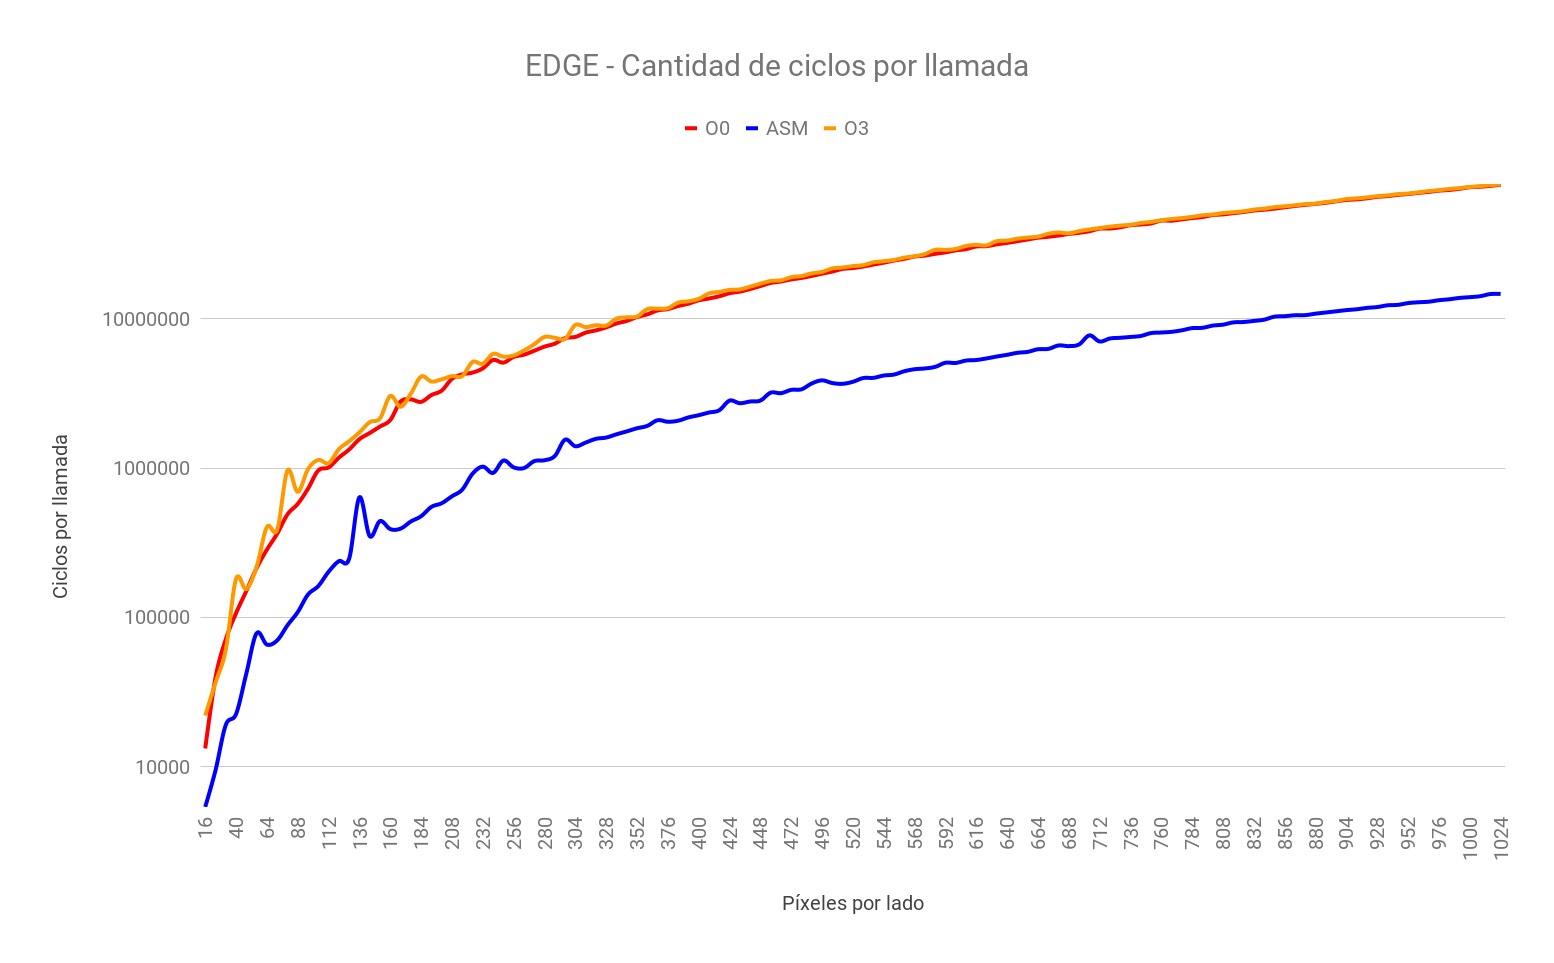
\includegraphics[width=0.45\textwidth]{imagenes/testperformance/EDGEperformanceLOG.png} \\
	  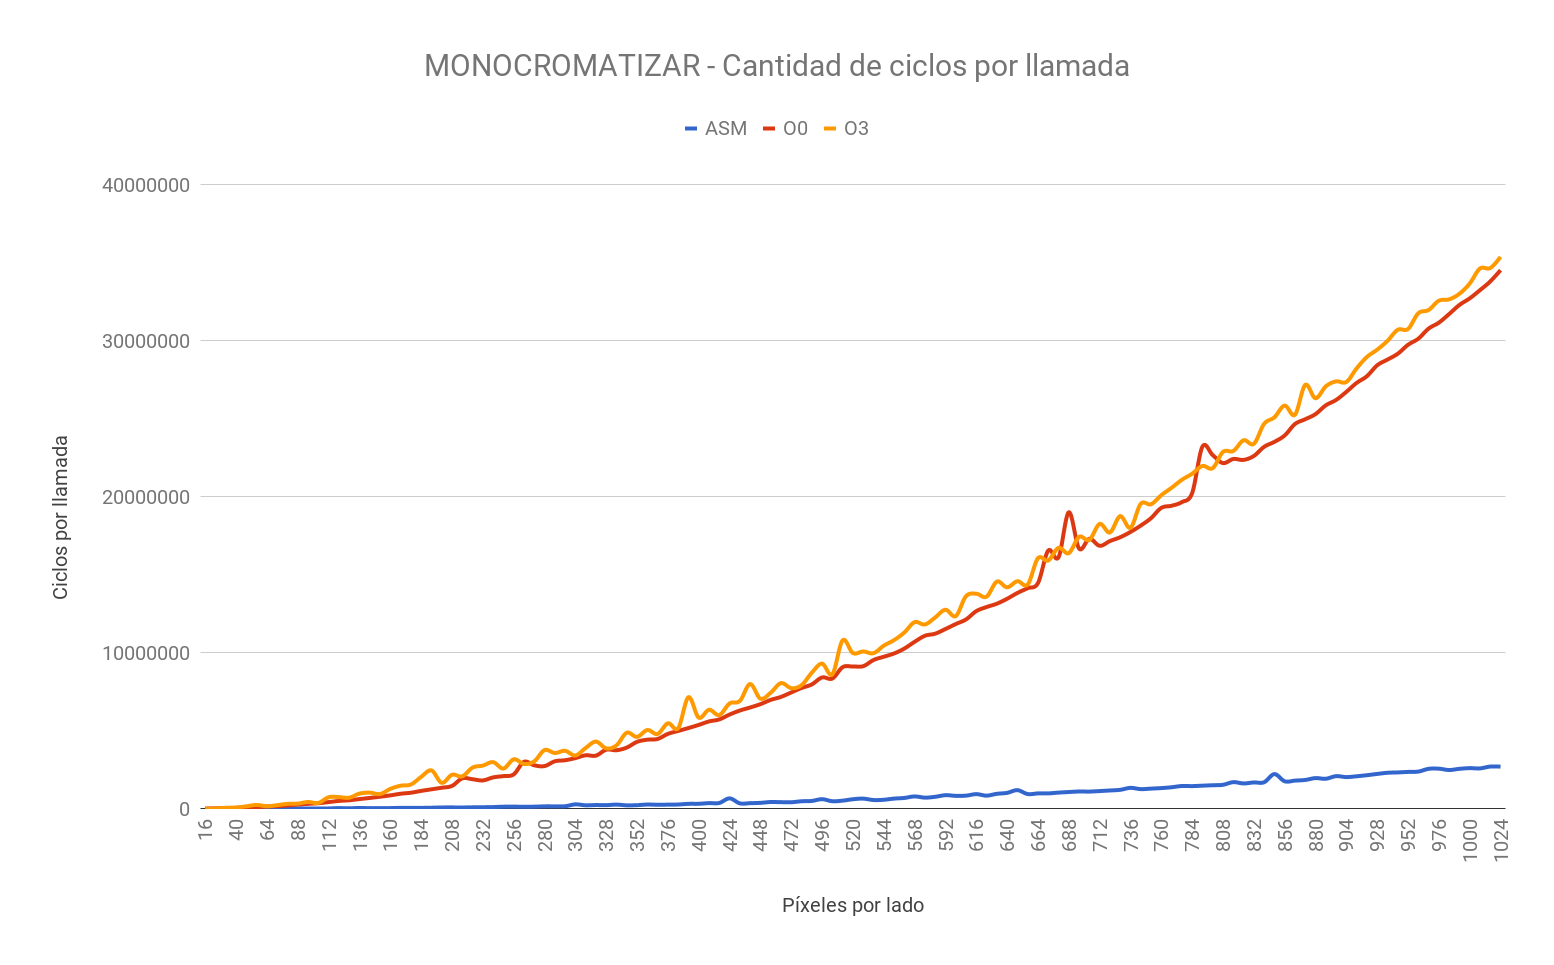
\includegraphics[width=0.45\textwidth]{imagenes/testperformance/MONOperformanceLIN.png} &
	  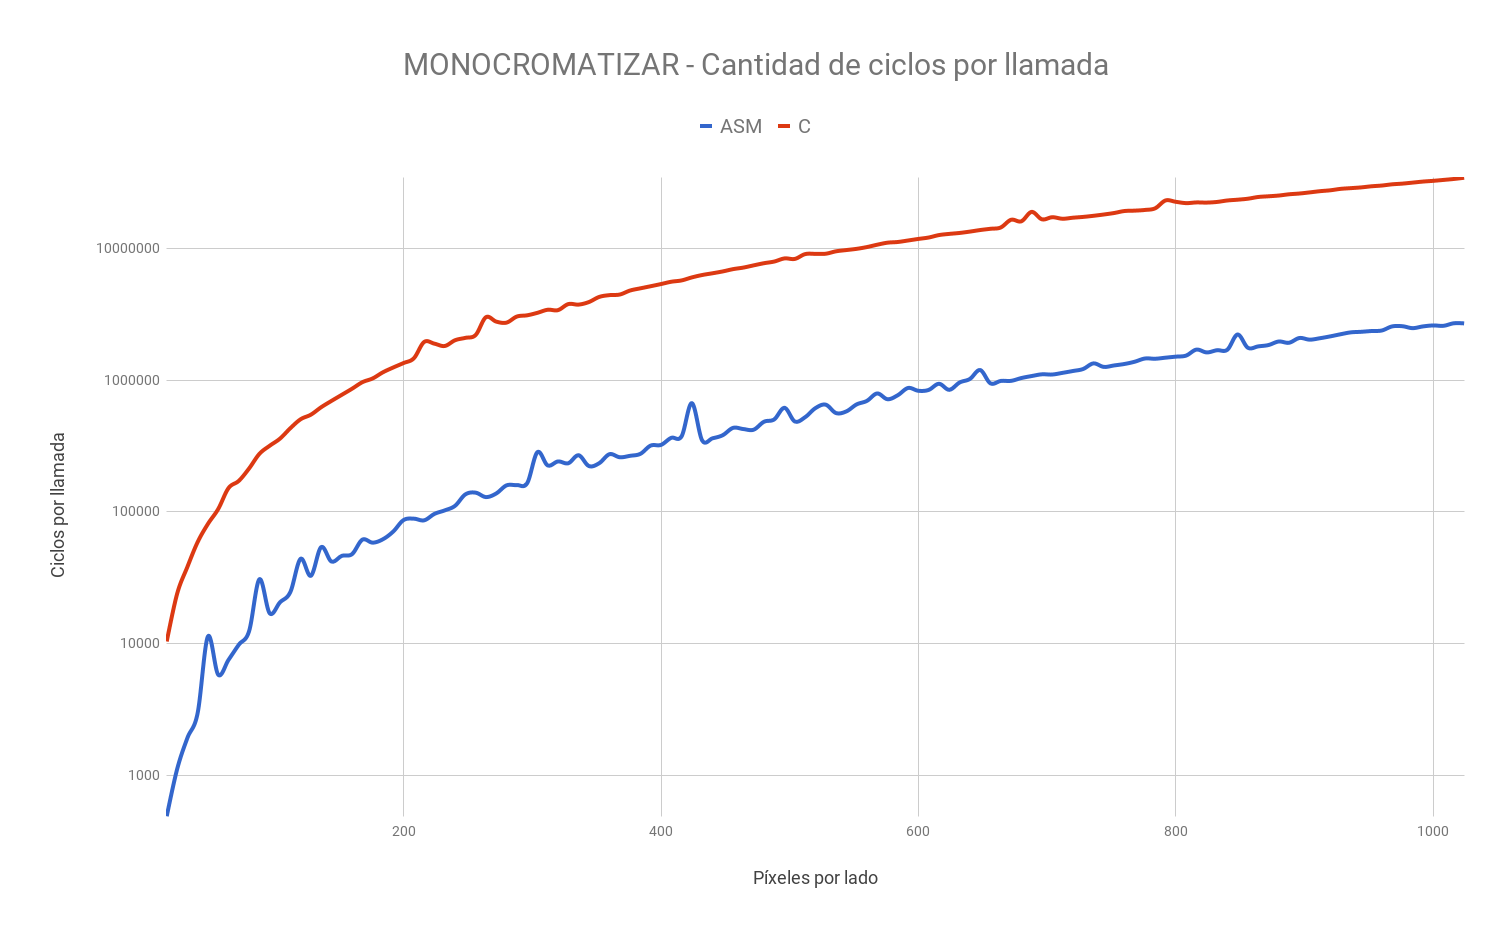
\includegraphics[width=0.45\textwidth]{imagenes/testperformance/MONOperformanceLOG.png} \\
	  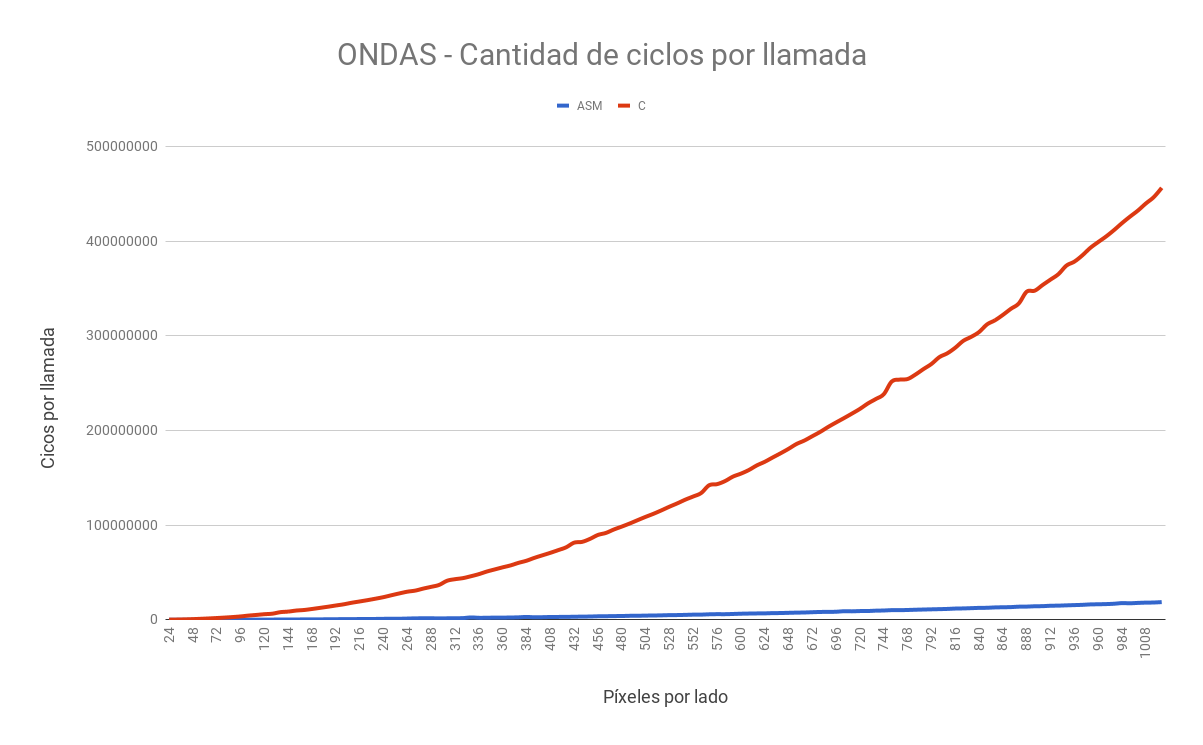
\includegraphics[width=0.45\textwidth]{imagenes/testperformance/ONDASperformanceLIN.png} &
	  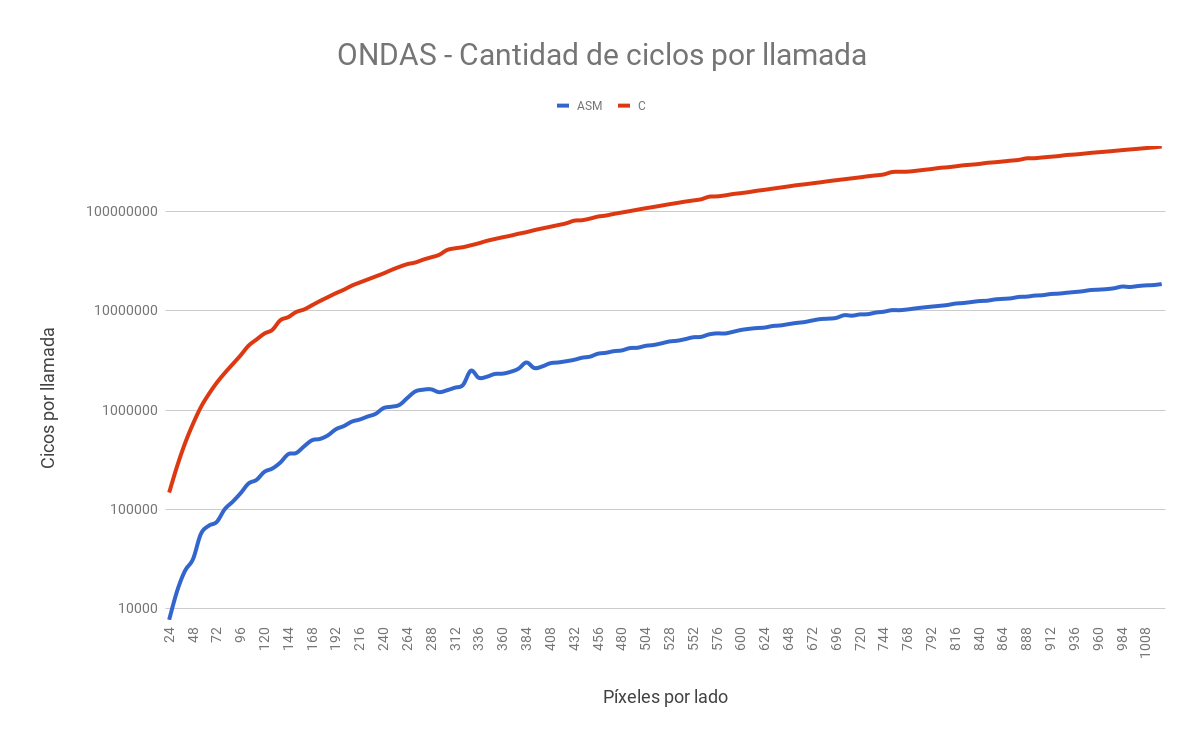
\includegraphics[width=0.45\textwidth]{imagenes/testperformance/ONDASperformanceLOG.png} \\
	  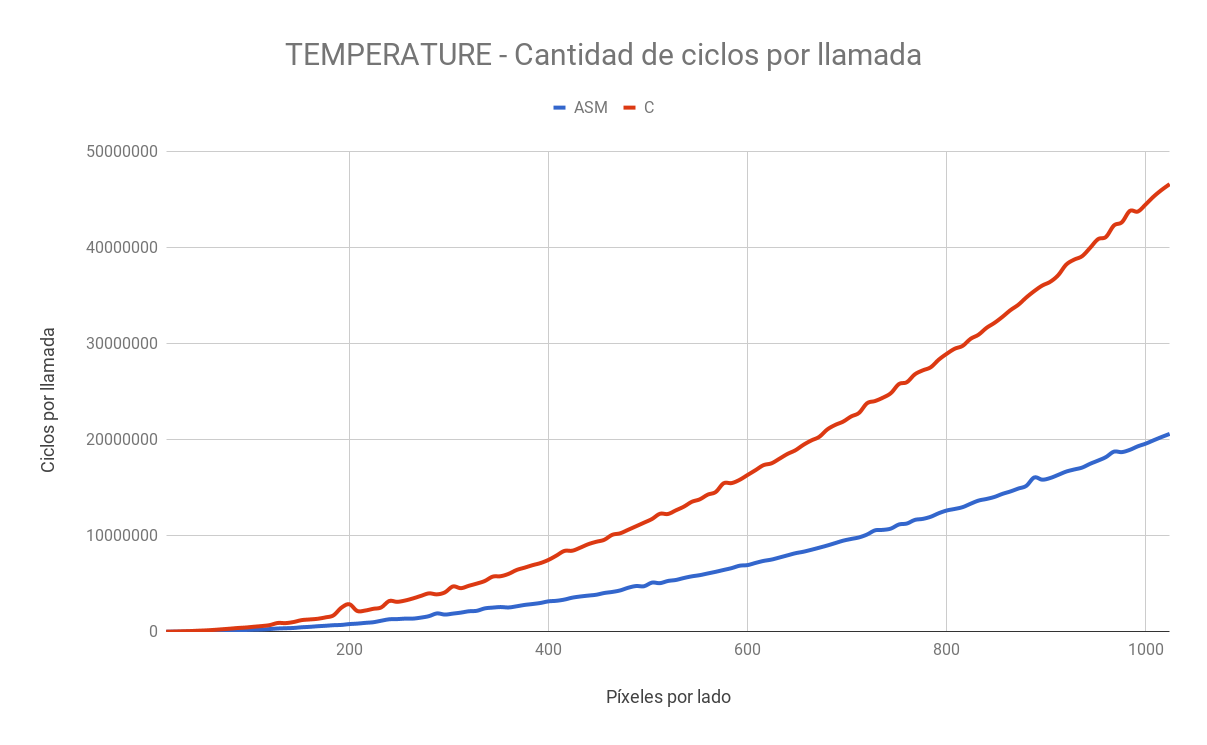
\includegraphics[width=0.45\textwidth]{imagenes/testperformance/TEMPperformance.png} &
	  \includegraphics[width=0.45\textwidth]{imagenes/testperformance/TEMPperformancelog.png} \\
	\end{tabular}
   \end{center}

\subsection{SIMD vs. SISD}

En la misma línea del experimento anterior quisimos evaluar las diferencias de tiempo entre el mismo algoritmo implementado en C, en ASM usando instrucciones SISD y en ASM con SIMD. La reescritura del código utilizando instrucciones SISD requirió 60 líneas de código, usando SIMD 30, y con C apenas 10; el tamaño de los archivos objeto pesó 2592B en SISD, 2608B en SIMD y 4280B en C.

\begin{center}

	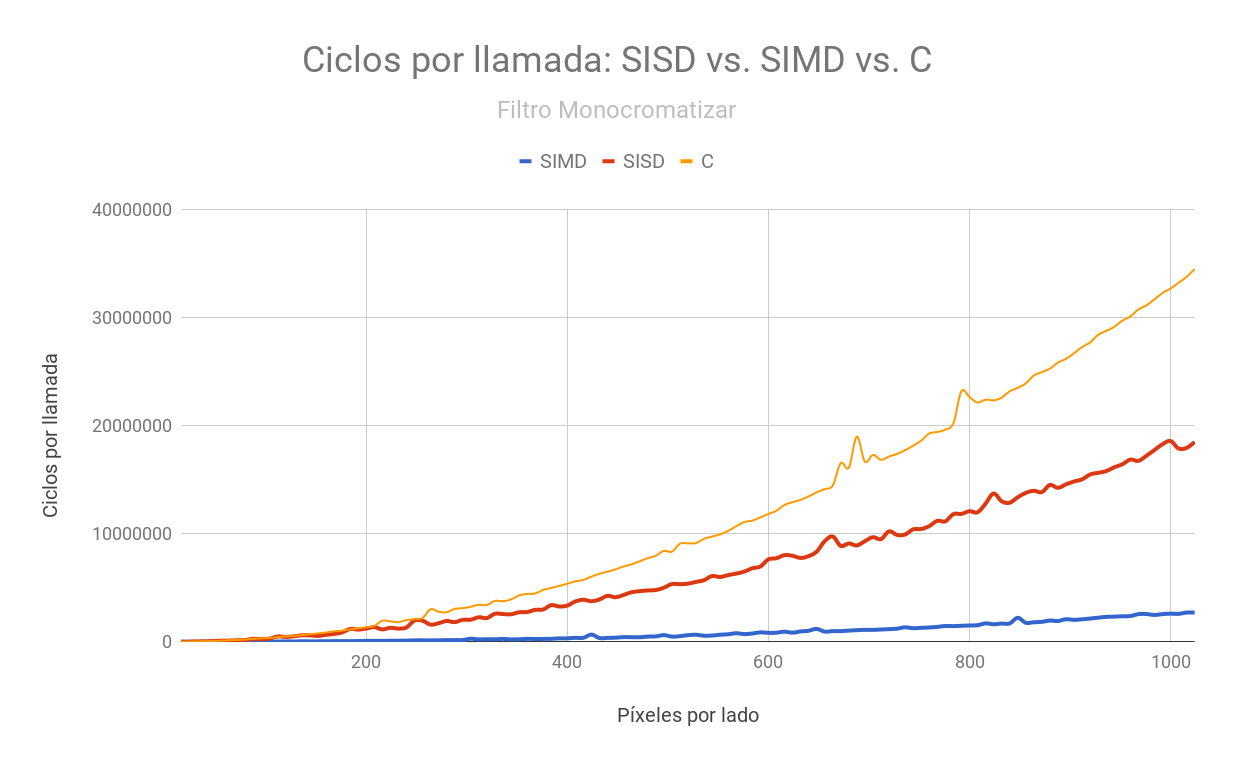
\includegraphics[width=0.9\textwidth]{imagenes/simdsisd/SIMDvsSISDvsClin.png} \\
	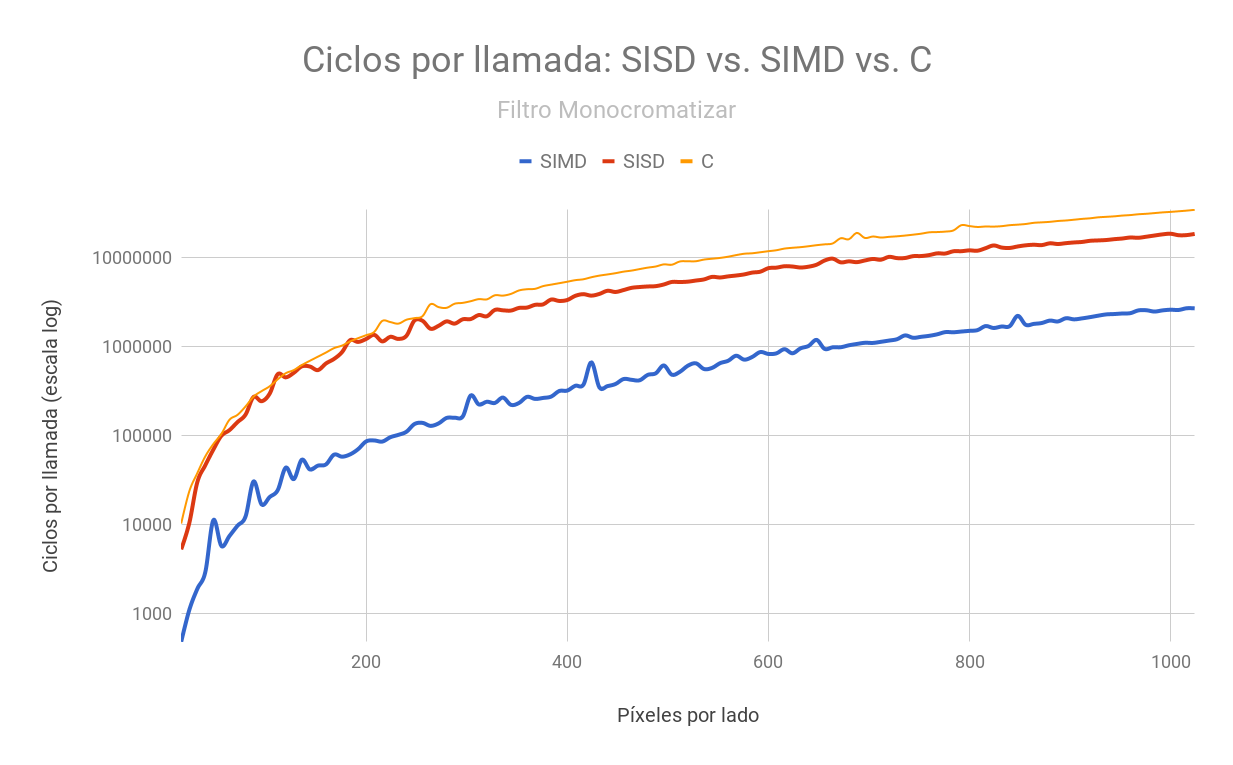
\includegraphics[width=0.9\textwidth]{imagenes/simdsisd/SIMDvsSISDvsClog.png}

\end{center}

Nuevamente pudimos apreciar como las instrucciones SIMD logran una superioridad en performance con respecto a la programación trabajando con datos secuencialmente. El mismo algoritmo implementado utilizando instrucciones SISD no logró imponerse sobre C para imagenes pequeñas -por debajo de los 256 píxeles por lado-, aunque sí lo logró para imagenes de mayor tamaño. En este caso el beneficio de trabajar en ASM puede verse opacado por la facilidad de la programación en C si no se utilizan las instrucciones SIMD. Sin embargo de mantenerse este crecimiento en la cantidad de llamadas para cada implementación, C sigue perdiendo cuando es más exigido.

\subsection{Branch Prediction}

\begin{center}
	\begin{tabular}{cccc}
	  
\includegraphics[width=0.45\textwidth]{imagenes/antiTEMP.jpg} &
	  
\includegraphics[width=0.45\textwidth]{imagenes/random.jpg} \\
	\end{tabular}
   \end{center}

\begin{center}

	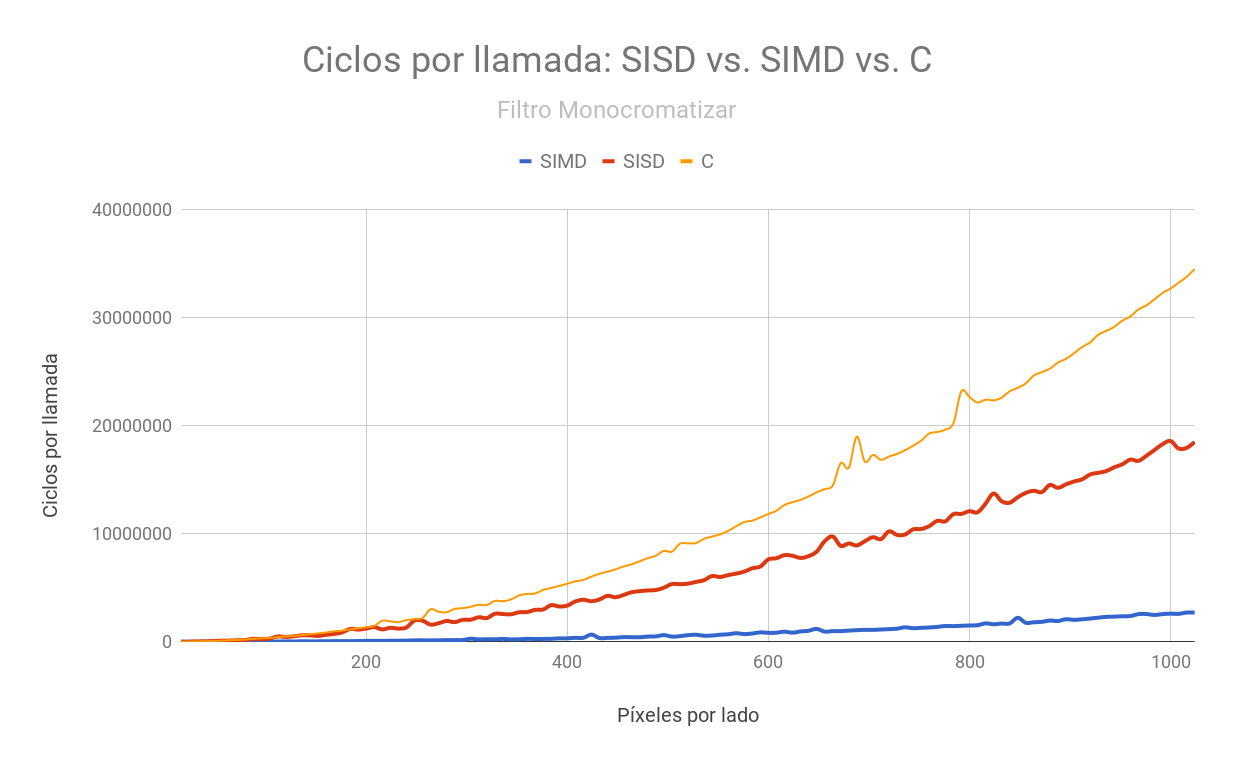
\includegraphics[width=0.9\textwidth]{imagenes/simdsisd/SIMDvsSISDvsClin.png} \\
	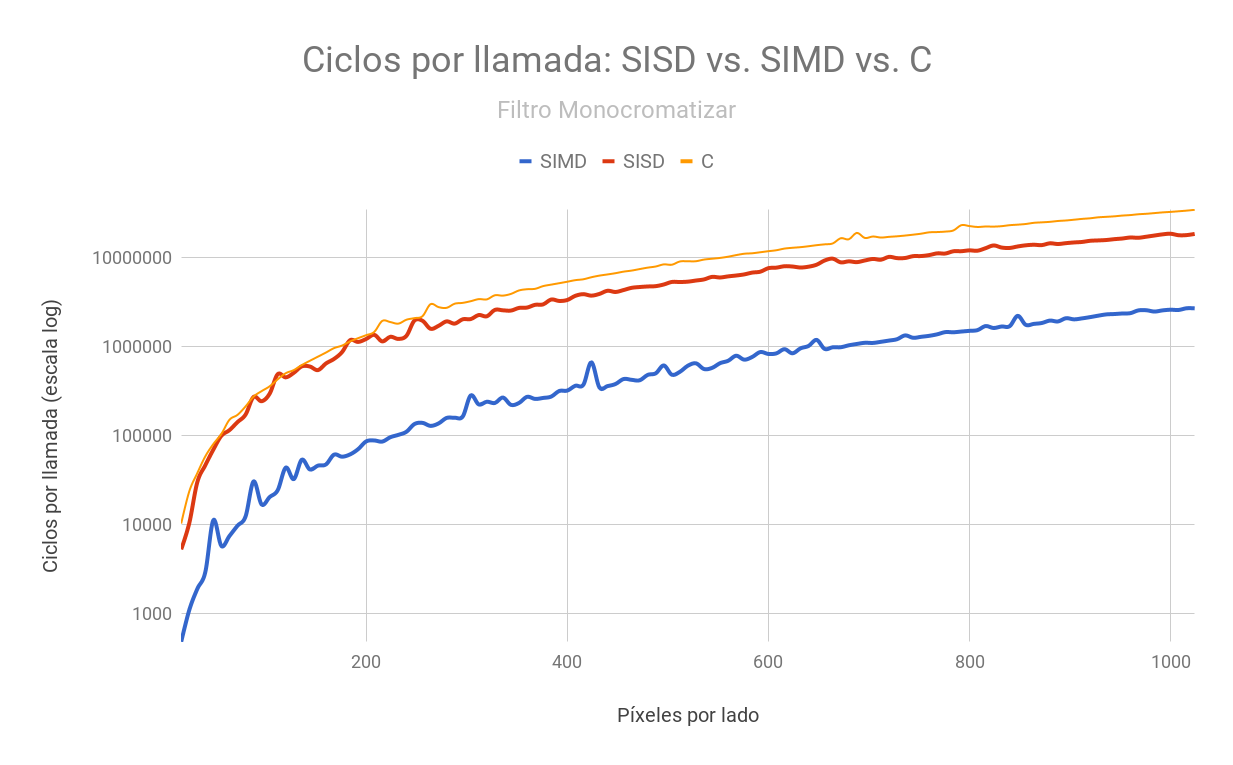
\includegraphics[width=0.9\textwidth]{imagenes/simdsisd/SIMDvsSISDvsClog.png}

\end{center}

\subsection{Loop Unrolling}

\begin{center}

	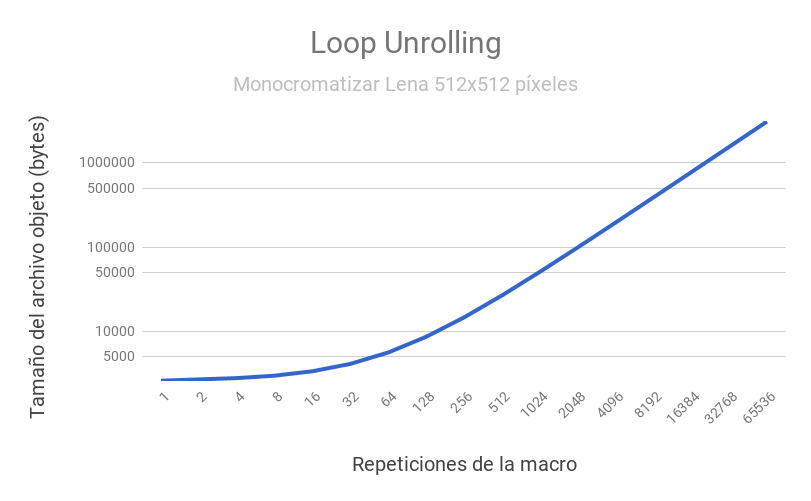
\includegraphics[width=0.9\textwidth]{imagenes/loopunrolling/size.png} \\
	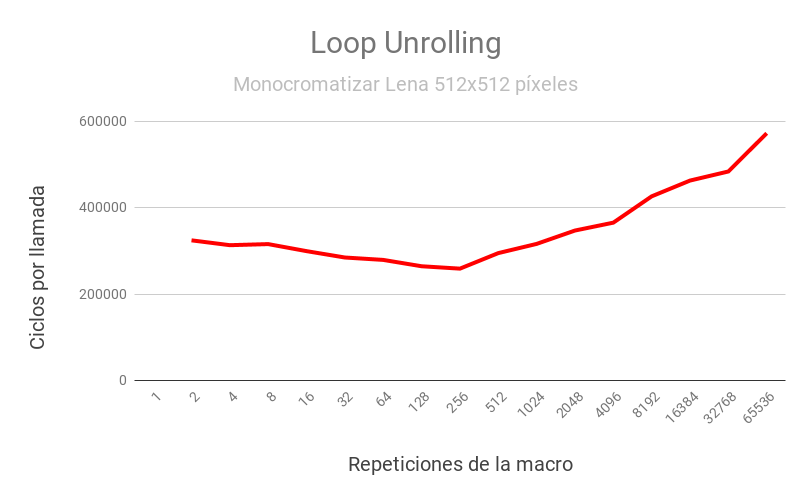
\includegraphics[width=0.9\textwidth]{imagenes/loopunrolling/time.png}

\end{center}

% La forma de medir el rendimiento de nuestras implementaciones se realizará por medio de la toma de tiempos de ejecución del algoritmo (sea este el codigo version asembler o el codigo C). Como los tiempos de ejecución son muy pequeños, se utilizará uno de los contadores de performance que posee el procesador.
% La instrucción de assembler rdtsc permite obtener el valor del Time Stamp Counter (TSC) del procesador. Este registro se incrementa en uno con cada ciclo del procesador. Obteniendo la diferencia entre los contadores antes y después de la llamada a la función, podemos obtener la cantidad de ciclos de esa ejecución. Esta cantidad de ciclos no es siempre igual entre invocaciones de la función, ya que este registro es global del procesador y se ve afectado por una serie de factores. \newline

% Existen principalmente dos problemáticas a solucionar:
% 1). La ejecución puede ser interrumpida por el scheduler para realizar un cambio de contexto,
% esto implicará contar muchos más ciclos (outliers) que si nuestra función se ejecutara sin
% interrupciones.

% 2). Los procesadores modernos varían su frecuencia de reloj, por lo que la forma de medir
% ciclos cambiará dependiendo del estado del procesador.
% \newline

% \textbf{solucion 1):} Para evitar el problema de los ciclos outliers lo que hicimos fue,

% \begin{itemize}
% 	\item[Paso 1:] En nuestro caso hicimos 100 veces la medición de tiempo de nuestro algoritmo y guardarlo en un contenedor(podría ser un arreglo,lista, conjunto, diccionario,.., etc).
% 	\item[Paso 2:] Sacar la media, tambien conocido como promedio, ejemplito:
% 		\begin{center} $ Prom =\frac{x_1+x_2+...+x_{100}}{100}$ \end{center}
% 		Donde $x_i$ es la medición de tiempo de la medición número $i$, con $1 \leq i \leq 100$ 
% 	\item[Paso 3:] Calculamos la varianza: 			
% 				\begin{center}
% 					$Varianza = \sigma^2 = \frac{(x_1 - Prom)+ (x_2 - prom)+ ...+ (x_{100} - prom)}{100} $
% 				\end{center}
% 	\item[Paso 4:] Calculamos el desvio estandar,  $\sigma = \sqrt{Varianza}$
% 	\item[Paso 5:] Utilizando el desvio estandar y el promedio, puedo ver que medición es "buena"  \\ y cual no. Más formalmente una medicion es "buena" si cumple: 
% 					\begin{center}
% 					$Prom - \sigma \leq x_i \leq Prom + \sigma $. %%\newline
% 					\end{center}
% 	 Luego sumando las todas las mediciones  "buenas" \\ y dividiendalas por la cantidad de mediciones buenas, obtengo el "promedio bueno". Con esto amortiguaria la cantidad de outliers de mis mediciones. 			
% \end{itemize}

% \textbf{Observar:} Todo lo anterior sirve también para mas de 100 mediciones. \newline

% \textbf{Solucion 2):} La solución que planteamos para esto fue, ejecutar sólamente el algoritmo. Con esto queremos decir que la ejecución estara en el nivel más alto de privilegio de ejecución. Esto lo hacemos metiendonos en el sistema operativo (en este caso ubuntu 14.04), tocando el monitor de sistema para darle privilegio a la ejecución. Tambien evitamos interumpir la maquina de forma mecanica(osea humana).  

\newpage
\section{Conclusiones y trabajo futuro}

    A partir de los experimentos realizados en este trabajo, se pudo llegar a la conclusión de que las ventajas que brinda el paradigma \textbf{SIMD} a la hora de implementar programas que realicen operaciones altamente paralelizables, como el procesamiento de imágenes, son verdaderamente significativas. Esto queda reflejado en la gran brecha de rendimiento que se observa entre las implementaciones realizadas con dicho paradigma y las que utilizan el lenguaje de programación C.

    Esto siempre debe contraponerse a otro hecho que se hizo presente durante el proceso de implementación: realizar un programa en lenguaje ensamblador resulta, por lo general, considerablemente más difícil que hacerlo en un lenguaje de más alto nivel. El código resultante es menos legible, es más sencillo cometer errores y el proceso de \emph{debugging} se vuelve considerablemente más arduo. Por eso es importante analizar de antemano las características del contexto particular de aplicación, para poder decidir si este esfuerzo adicional realmente vale la pena.

    Ahondando en los detalles más técnicos de la implementación, se intentó la realización de una optimización manual dentro del código ensamblador, sin obtener resultados destacables. La razón de esto es que estructura del código dificultaba ampliamente la realización de dicha modificación. Realizar la optimización de manera efectiva habría implicado modificar gran parte del código ya armado, con un costo casi equivalente al de empezarlo de nuevo con un enfoque distinto; esto es consecuencia de la ya mencionada dificultad que presenta mantener el código programado en este lenguaje.


\end{document}